\documentclass[12pt,a4paper]{article}

\usepackage{lastpage}
\usepackage{graphicx}
\usepackage{tabularx}
\usepackage{longtable}
\renewcommand{\arraystretch}{1.6}

\usepackage{relsize}

\usepackage{listings}
\usepackage{color}
\definecolor{dkgreen}{rgb}{0,0.6,0}
\definecolor{gray}{rgb}{0.5,0.5,0.5}
\definecolor{mauve}{rgb}{0.58,0,0.82}
\lstset{frame=tb,
  language=Java,
  aboveskip=3mm,
  belowskip=3mm,
  showstringspaces=false,
  columns=flexible,
  basicstyle={\small\ttfamily},
  numbers=none,
  numberstyle=\tiny\color{gray},
  keywordstyle=\color{blue},
  commentstyle=\color{dkgreen},
  stringstyle=\color{mauve},
  breaklines=true,
  breakatwhitespace=true,
  tabsize=3,
  morecomment=[l][basicstyle]{http://},
  morecomment=[l][basicstyle]{https://},
  literate={~} {$\sim$}{1}
}

%reference of section names
\usepackage{nameref}


\usepackage[total={160mm, 210mm},headheight=50pt]{geometry}

\usepackage[usenames, dvipsnames]{xcolor}
\usepackage{sectsty}
\allsectionsfont{\color{blue}\normalfont\sffamily}

\usepackage{amsmath}
\usepackage[adobe-utopia]{mathdesign}
\usepackage[T1]{fontenc}

\usepackage{wallpaper}

%wavy underlines% % % % %
\usepackage{ulem} 

%highlight % % % % %
\usepackage{soul} 
\usepackage{tikz}
\usetikzlibrary{calc}
\usetikzlibrary{decorations.pathmorphing}

\makeatletter

\newcommand{\defhighlighter}[3][]{%
  \tikzset{every highlighter/.style={color=#2, fill opacity=#3, #1}}%
}

\defhighlighter{yellow}{.5}

\newcommand{\highlight@DoHighlight}{
  \fill [ decoration = {random steps, amplitude=1pt, segment length=15pt}
        , outer sep = -15pt, inner sep = 0pt, decorate
        , every highlighter, this highlighter ]
        ($(begin highlight)+(0,8pt)$) rectangle ($(end highlight)+(0,-3pt)$) ;
}

\newcommand{\highlight@BeginHighlight}{
  \coordinate (begin highlight) at (0,0) ;
}

\newcommand{\highlight@EndHighlight}{
  \coordinate (end highlight) at (0,0) ;
}

\newdimen\highlight@previous
\newdimen\highlight@current

\DeclareRobustCommand*\highlight[1][]{%
  \tikzset{this highlighter/.style={#1}}%
  \SOUL@setup
  %
  \def\SOUL@preamble{%
    \begin{tikzpicture}[overlay, remember picture]
      \highlight@BeginHighlight
      \highlight@EndHighlight
    \end{tikzpicture}%
  }%
  %
  \def\SOUL@postamble{%
    \begin{tikzpicture}[overlay, remember picture]
      \highlight@EndHighlight
      \highlight@DoHighlight
    \end{tikzpicture}%
  }%
  %
  \def\SOUL@everyhyphen{%
    \discretionary{%
      \SOUL@setkern\SOUL@hyphkern
      \SOUL@sethyphenchar
      \tikz[overlay, remember picture] \highlight@EndHighlight ;%
    }{%
    }{%
      \SOUL@setkern\SOUL@charkern
    }%
  }%
  %
  \def\SOUL@everyexhyphen##1{%
    \SOUL@setkern\SOUL@hyphkern
    \hbox{##1}%
    \discretionary{%
      \tikz[overlay, remember picture] \highlight@EndHighlight ;%
    }{%
    }{%
      \SOUL@setkern\SOUL@charkern
    }%
  }%
  %
  \def\SOUL@everysyllable{%
    \begin{tikzpicture}[overlay, remember picture]
      \path let \p0 = (begin highlight), \p1 = (0,0) in \pgfextra
        \global\highlight@previous=\y0
        \global\highlight@current =\y1
      \endpgfextra (0,0) ;
      \ifdim\highlight@current < \highlight@previous
        \highlight@DoHighlight
        \highlight@BeginHighlight
      \fi
    \end{tikzpicture}%
    \the\SOUL@syllable
    \tikz[overlay, remember picture] \highlight@EndHighlight ;%
  }%
  \SOUL@
}
\makeatother
% % % % % % % % % %

\usepackage{xargs}          
\usepackage[colorinlistoftodos,prependcaption,textsize=scriptsize,textwidth=2cm]{todonotes} 
\newcommandx{\unsure}[2][1=]{\todo[linecolor=red,backgroundcolor=red!25,bordercolor=red,#1]{#2}}
\newcommandx{\change}[2][1=]{\todo[linecolor=blue,backgroundcolor=blue!25,bordercolor=blue,#1]{#2}}
\newcommandx{\info}[2][1=]{\todo[linecolor=OliveGreen,backgroundcolor=OliveGreen!25,bordercolor=OliveGreen,#1]{#2}}
\newcommandx{\improvement}[2][1=]{\todo[linecolor=Plum,backgroundcolor=Plum!25,bordercolor=Plum,#1]{#2}}
\newcommandx{\thiswillnotshow}[2][1=]{\todo[disable,#1]{#2}}

\newcommandx{\yilin}[2][1=]{\todo[linecolor=yellow,backgroundcolor=yellow!25,bordercolor=yellow,#1]{#2}}

% % % % % % % % % % %
\usepackage{fancyhdr}
\pagestyle{fancy}
\fancyhead{}
\fancyfoot{}
\fancyhead[L]{%
	\footnotesize{%
		FP7-SMARTCITIES-2013 $|$ ICT-2013.6.4 $|$ GA 608774 \\
		Deliverable 3.3 \\
		Page \thepage  /\pageref{LastPage}
		\vspace{1cm}
	} 
}
\fancyhead[R]{ %
	
\includegraphics[height=2.5cm]{./logos/civis_rgb.jpg}
}
\fancyfoot[L]{%
	\vspace{-15pt}
	\footnotesize{Version: 1.1;  Version Date: Jun 30, 2016}
}
\fancyfoot[R]{ %
	\vspace{-15pt}
	
\includegraphics[height=1.5cm]{./logos/FP7-gen-RGB.jpg}
	
\includegraphics[height=1.5cm]{./logos/flag_yellow_high.jpg}\\
	\color{Gray}\scriptsize{CIVIS project has received research\\
							funding from the European Union}
}
\renewcommand{\headrulewidth}{0pt}
%\renewcommand{\footrulewidth}{0.4pt}

\setlength\headheight{90pt}
%\addtolength{\textheight}{-20.8pt}

\renewcommand*\contentsname{Table of Contents}

\usepackage{natbib}

\usepackage[hyphens]{url}
\usepackage[colorlinks]{hyperref}
\hypersetup{
    allcolors=blue,
}

\usepackage{enumitem}

% % % % % % % %\subsubsubsection
\usepackage{titlesec}
\setcounter{secnumdepth}{4}

\titleformat{\paragraph}
{\normalfont\normalsize\bfseries}{\theparagraph}{1em}{}
\titlespacing*{\paragraph}
{0pt}{3.25ex plus 1ex minus .2ex}{1.5ex plus .2ex}

\begin{document}

\ThisCenterWallPaper{.8}{./logos/civis.png}


\begin{titlepage}

  \begin{center}
	
	\vspace*{-1.5cm}
    {\fontsize{36}{32}\usefont{OT1}{phv}{m}{n}\selectfont\color{RedOrange}
        D3.3 Final Field Tested Integrated Energy System 
        \\ \vspace{.5cm}
		Workpackage 3
    }
	
	 \vfill
	 
    {\fontsize{18}{22}\usefont{OT1}{phv}{m}{n}\color{RedOrange}
      Responsible Unit:  TU Delft
      \\ \vspace{.3cm}
      Authors: Y. Huang, G. Poderi, L.Y. Yishagerew, H. Hasselqvist, A.~Massaro, S. Scepanoic, H. Ensing, F. Cuscito
    }

  \end{center}

\end{titlepage}


\addtolength{\wpXoffset}{-7.2cm}
\CenterWallPaper{.62}{./logos/civis2.png}


\section*{Document technical details}

\begin{tabularx}{\textwidth}{|X|X|}
\hline
Document Number	& D3.3 \\ \hline
Document Title	&  Integrated Energy System\\ \hline
Version	&  1.3\\ \hline
Status	 &  Final \\ \hline
Work Package		&  3\\ \hline
Deliverable Type 	&  R/T \\ \hline
Contractual Date of delivery 	&  01/10/2015 \\ \hline
Actual Date of Delivery		&  07/10/2015 \\ \hline
Responsible Unit	&  TU Delft \\ \hline
Contributors & CN, KTH, AALTO, KIT \\ \hline
Keywords List &  social smart grid platform, design, mock-up, prototype\\ \hline
Dissemination Level	&  PU \\ \hline
\end{tabularx}

\clearpage

\section*{Document changelog}

{
\begin{tabularx}{\textwidth}{|l|l|l|>{\raggedright\arraybackslash}p{4cm}|X|}
\hline
\textbf{Version}	& \textbf{Date} &	\textbf{Status} &	\textbf{Author (Unit)} &	\textbf{Description}  \\ \hline
0.1 & May 12, 2016 & Outline & Y. Huang (TU Delft) & The first outline\\ \hline
0.2 & May 13 & Draft & Y. Huang (TU Delft) &  2.1; 2.2; 2.3.1\\ \hline
0.x & \today & Outline & Y. Huang (TU Delft) &  \\ \hline

\end{tabularx}
}




\section*{CIVIS Consortium}
CIVIS (Grant Agreement contract No. 608774) is a Collaborative Project within the 7th Framework Programme, theme FP7-SMARTCITIES-2013, ICT-2013.6.4. As defined in the Consortium Agreement [2], members of the Consortium are:

\vspace{.2cm}

\begin{longtable}{|c|p{14.5cm}|}
\hline
\textbf{No.} & \textbf{Beneficiaries} \\ \hline
1 &	UNIVERSITA DEGLI STUDI DI TRENTO, established in VIA CALEPINA 14, 38122 TRENTO - ITALY, represented by Mr Paolo COLLINI, Rector, or his authorised representative, the beneficiary acting as coordinator of the consortium (the "coordinator"). \\ \hline
2 &	AALTO-KORKEAKOULUSAATIO established in OTAKAARI 1, 00076 AALTO -
FINLAND, represented by Mr Ilkka NIEMEL\"{A}, Deputy President and/or Mr Tuija PULKKINEN,
Vice President, or their authorised representative. \\ \hline
3 &	FONDAZIONE CENTRO STUDI ENEL established in VIALE REGINA MARGHERITA 137, 00198 ROMA - ITALY, represented by Mr Francesco STARACE, President, or his authorised representative. \\ \hline
4 &	IMPERIAL COLLEGE OF SCIENCE, TECHNOLOGY AND MEDICINE established
in Exhibition Road, South Kensington Campus, SW7 2AZ LONDON - UNITED KINGDOM, represented by Ms Carole MEADS, Senior Negotiator, European Policy and/or Mr James LLOYD, Contracts Administrator (Europe), or their authorised representative. \\ \hline
5 &	INSTITUTO SUPERIOR TECNICO established in Avenida Rovisco Pais 1, 1049-001 LISBOA - PORTUGAL, represented by Mr Arlindo OLIVEIRA, President, or his authorised representative. \\ \hline
6 &	Karlsruher Institut fuer Technologie established in Kaiserstrasse 12, 76131 Karlsruhe - GERMANY, represented by Mr Bernhard DASSELAAR, Head of Cost and Fund Management and/or Mr Wolf FICHTNER, Head of IIP, or their authorised representative. \\ \hline
7 &	KUNGLIGA TEKNISKA HOEGSKOLAN established in BRINELLVAGEN 8, 100 44
STOCKHOLM - SWEDEN, represented by Mr Peter GUDMUNDSON, President and/or Mr Kenneth BILLQVIST, Head of Research Office, or their authorised representative. \\ \hline
8 &	SANTER REPLY SPA established in VIA ROBERT KOCH 1/4, 20152 MILANO - ITALY, represented by Mr Luigi CICCHESE, Partner, or his authorised representative. \\ \hline
9 &	NEDERLANDSE ORGANISATIE VOOR TOEGEPAST NATUURWETENSCHAPPELIJK ONDERZOEK - TNO established in Schoemakerstraat 97, 2600 JA DELFT - THE NETHERLANDS, represented by Drs. Ren\'{e} HOOIVELD, Director of Sustainable
Energy, or his authorised representative. \\ \hline
10 &	TECHNISCHE UNIVERSITEIT DELFT established in Stevinweg 1, 2628 CN DELFT - THE NETHERLANDS, represented by Mr Jeroen VAN DEN HOVEN, Dean and/or Mr Hans DE BRUIJN, Vice-Dean, or their authorised representative. \\ \hline
11 &	CREATE-NET (CENTER FOR RESEARCH AND TELECOMMUNICATION
EXPERIMENTATION FOR NETWORKED COMMUNITIES) established in VIA ALLA CASCATA 56/D, 38123 TRENTO - ITALY, represented by Mr Imrich CHLAMTAC, President, or his authorised representative. \\ \hline
12 &	FONDAZIONE BRUNO KESSLER established in VIA SANTA CROCE 77, 38122
TRENTO - ITALY, represented by Mr Andrea SIMONI, General Secretary and/or his authorised representative. \\ \hline
\end{longtable}

\clearpage


{\hypersetup{linkcolor=black}
\tableofcontents}


\section*{Executive Summary}
\addcontentsline{toc}{section}{Executive Summary}

This report summarizes the 3rd year's activities of CIVIS WP3 and the results and contributions of the WP. The research attention of CIVIS is oriented towards the potentials and challenges of users' collective action, social values and sense of communities in smart grids. To this end, the main activities in the 3rd year of WP3 continued the iterative, theory-driven, and user-centered development process in the 3rd year. WP3 completed the design and development of the CIVIS \textit{YouPower} platform, expanding upon the 2nd year's results.

The design and development of YouPower can be divided into three self-contained, interrelated and composable parts: (1) Action Suggestions (contextualized and deployed to both test sites); (2) Housing Cooperatives (contextualized and deployed to the Swedish test site); and (3) Energy Awareness at Individual and Collective Levels (contextualized and deployed to the Italian test site). The intension of the application is to increase energy awareness, to inform users' energy consumption know-how, to promote environmental social norms, and to facilitate users for energy conservation and load-shifting behavior changes that are implementable in everylife. We derived ten design guidelines to address a number of design issues based on (pro-environmental interventions, social and environmental psychology) literature and our design experience. These guidelines are discussed in depth in this report and they can be useful for a wide group of environmental intervention designers: 
\begin{enumerate}
\item Develop and enhance consumers' energy conservation know-how through action suggestions
that are implementable in everyday life.
\item Explicitly express action suggestions with concrete and reliable content.
\item Provide suggestions ranging from one-time actions to routine actions.
\item Support demand side management (load-shifting) through simple time-of-use (ToU) signals.
\item Indicate the effort entailed by a suggested action and its potential impact in an understandable way.
\item Enhance and maintain intrinsic motivation; promote more active and volitional forms
of extrinsic motivation.
\item Use social norms and public commitment to address low motivation.
\item Facilitate consumers to reflect on (environmental) lifestyle choices in the process
of behavior change.
\item Engage all household members.
\item Define energy interventions through co-design approaches.
\end{enumerate}

The key features designed for the YouPower platform include: 

\begin{enumerate}
\item Action suggestions, where users are provided with suggestions of actions that are implementable in everyday household practices. 
% 
It presents users with motivators for behavior change (and its process), and means for self-monitoring, self-reflection and social sharing of the pro-environmental behavior change process at individual, household and community levels. 
Each action is accompanied with the information about the potenial effort and impact, user comments and a list of participants who are taking this action. A user can decide whether to take an action and to schedule it. A user also see actions of household members. 

\item Housing cooperatives, where energy management and cooperative energy reduction actions are linked to each cooperative's energy performance. 
% 
The building level energy information and the energy related actions of each housing cooperative are presented to users. This allows comparison between housing cooperatives based on the energy performance and actions, and supports knowledge exchange and social sharing and learning among cooperatives in energy reduction actions.

\item Energy awareness at individual and collective levels, where users are presented with real time and historical energy consumption and production information. 
% 
It provides users with time-of-use signals based on real time and forecasted information about local production from renewable sources and the corresponding energy demand in order to enable load-shifting actions in everyday practice. It also presents users with reference information about energy performance in relation to the neighborhoods. 

\end{enumerate}

The CIVIS YouPower platform is currently being deployed and tested at the Stockholm (Sweden) and Trento (Italy)
test sites corresponding to the local context. To reach a wide group of research communities and general public, the YouPower software is open source with an online repository and API documentation. The package management and application setup of YouPower are also discussed in this report to support potential usership and future development of the application. 




\section{Introduction}

\subsection{Overview}

\begin{quote}
D3.2) Final field tested Integrated Energy System: Output of T3.1-5; Based on information provided by the deployment of deliverable 3.2 the software is further refined to provide energy services and community management (open source). 
\end{quote}

In the third year of Work Package 3 (WP3), we continued the design and development of the software platform YouPower\footnote{ \url{http://civis.tbm.tudelft.nl/}} expanding the results reported in D3.2. In this report, the final results are summarized as a whole for readability and usefulness. The refinement and improvement made in the third year are highlighted where necessary when possible. 
% 
The functionalities of the platform reported are deployed at Stockholm and Trento test sites respectively according to the local context. The YouPower software is open source under the Apache v.2 License\footnote{\url{https://github.com/CIVIS-project/YouPower/blob/master/LICENSE}}. It has  an online repository at GitHub\footnote{ \url{https://github.com/CIVIS-project/YouPower/}}. 
The backend API documentation is aslo available online\footnote{ \url{http://civis.tbm.tudelft.nl/apidoc/}}. 

...

%\subsection{Aims and Scope}

As stated in D3.2 \citep{Huang2015c}, the CIVIS platform is composed of two parts: the CIVIS back-end services, and the CIVIS front-end application with which users directly interact (Figure~\ref{fig:platform}). 
%
\begin{figure}
\begin{center}\footnotesize
	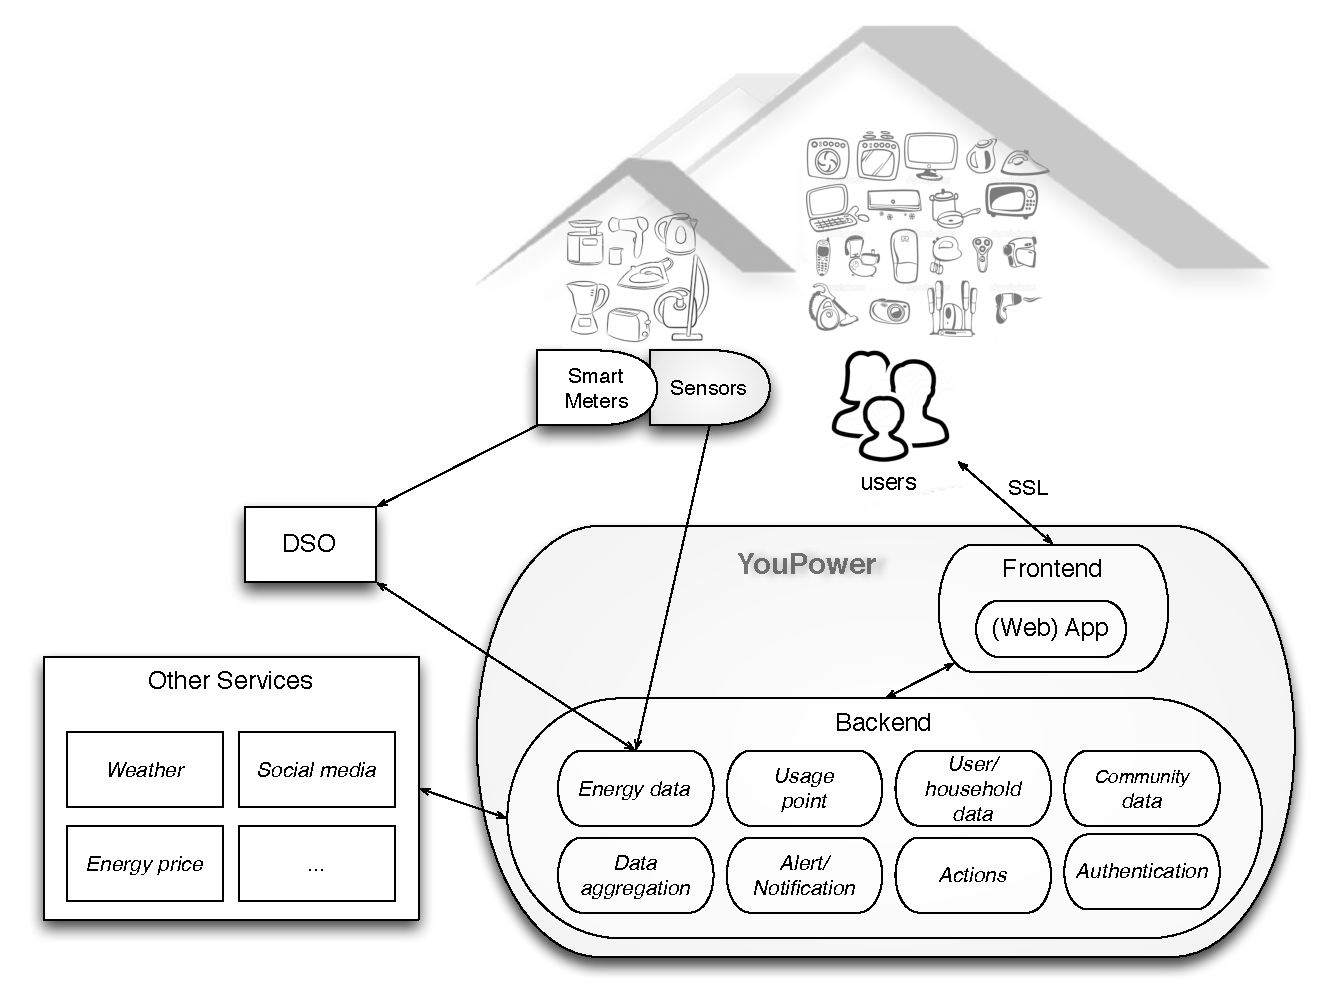
\includegraphics[width=.95\textwidth]{img/civis_platform_overview.pdf}\\
	DSO (Distribution System Operators),  SSL (Secure Sockets Layer)
	\caption{CIVIS platform overview}\label{fig:platform}
\end{center}
\end{figure}
% 
WP4 focuses on the system level ICT services that deal with energy data collected by smart meters and sensors at the Swedish and Italian test sites (see D4.3 for more details). 
WP3 focuses on the front-end application and the social level ICT services that deal with data related to user, household, community, action suggestions, etc. Unless otherwise specified, this report discusses the design and development of the WP3 part of the CIVIS platform which is called YouPower. (The CIVIS front-end application used to be called EnergyUP. The old name may be found in some old documents and/or mock-ups.)

... 

Environmental problems have their origins in human behavoir, and as a result, any solution to enviromental issues will require changes in behavoir 
\citep{Schultz2014}.
%The authentication of user sign up and login to an EnergyUP account is managed by WP3 services. A user may also choose to link his or her energy data, additional authentication is required. 

%The effectiveness of smart grids depends on consumer engagement and action. Today’s consumers have a vague understanding of the grid. How consumers understand the smart grid will shape how they feel about it, and in turn how readily they adopt it, and how they use it. 
%
%Seeing is believing 
%If consumers are given useful feedback on how they use energy and are provided with recommendations on how to improve, they will have the chances to make more informed energy choices. 
%
%

\subsection{Design and Development: the Continuation}

The design and development of YouPower is theory-driven, user-centered and iterative. We researched literature on intervention strategies and social smart grid applications directed at promoting pro-environmental consumer behavior change. This provided an initial set of design ideas that are iteratively refined and improved through the design process. Applying a user-centered design process can lead to more acceptable, satisfying and effective designs \citep{Brynjarsdottir2012}. This increases the potential of the intervention \citep{dick2012empowering} and may help increase user engagement with respect to the sense of relatedness to the application \citep{pierce2003state,schwartz2014people,edward2015review}. 

In the second year of CIVIS, we started with brainstorming sessions and a design workshop. A set of features was prototyped in simple handcrafted mock-ups used as a basis for discussion, and then underwent iterative rapid prototyping which produced wireframes as visual guides that can be more effectively communicated to general users. These prototypes were evaluated by user tests with groups of students and colleagues. Using the wireframe prototypes and later the software prototypes, we conducted focus group studies with consumers in Trento, test studies and focus groups with consumers and housing cooperative members in Stockholm, as well as a user study with pro-environmental participants in Helsinki. 

In the third year of CIVIS, the design and development continued. We have paid particular attention to quick responses to changes, and adaptive development. We also furthered literature research in environmental psychology and intervention design, and expanded the design guidelines based on our design practices and experiences. These guidelines can be useful for a wider group of designers interested in pro-environmental intervention.   .... >>>Any events in the third year?<<< ...   YouPower had been refined and improved gradually in the third year resulting in the current version of the application, which is deployed at Stockholm and Trento test sites. The rest of this report presents and discusses the latest version of YouPower. 

%literature, group feedback (internal), user feedback: workshops, focus groups 
 


\section{CIVIS Platform Design}

\subsection{Motivation: Bridging the Attitude-Behavior Gap}

Environmentally significant behaviours should be understood as relatively inconspicuous actions performed in the context of everyday life \citep{Burgess2008}. People consume energy through many daily practices and routines in households \citep{Burgess2008,Hargreaves2010, Fehrenbacher2011,Burchell2014}. How and to what extent these daily actions affect domestic energy use and in turn the environment are not always readily apparent to average consumers  \citep{Burgess2008,Delmas2013}. This knowledge deficit poses significant constraints for consumers to perform and engage in energy conservation (and energy efficiency) behaviors \citep{Schultz2002,Burchell2014}. Acquiring such information is often costly  \citep{Delmas2013}. 

A rich body of empirical research suggests that relevant information tends to result in higher knowledge levels but not necessarily in behavior changes or energy savings  \citep{Abrahamse2005,Delmas2013,Burchell2014,Asensio2015}. Despite growing environmental awareness and articulated preference for ``green'' lifestyles, people's environmental values and attitudes often fail to materialize in actual actions and behavior changes, from energy conservation, to recycling,  to the purchase of green products  \citep{Schultz2002,Abrahamse2005,Claudy2013}. This imparity is commonly referred to as the attitude-behavior gap or the value-action gap  \citep{Blake1999,Kollmuss2002,Claudy2013}. 

Although there is no single framework or theory that provides definitive explanations for the attitude-behavior gap  \citep{Kollmuss2002,Schultz2014}, literature provides suggestions that shed some light on this issue. People perform (or do not perform) certain pro-environmental actions for many reasons  \citep{Schultz2002}. The reasons for acting are often referred to as motives or motivation  \citep{Parfit1997,Moisander2007}. A distinction can be made between \textit{primary motives} and \textit{selective motives}  \citep{Kollmuss2002,Moisander2007}. Primary motives influence decisions to engage (or not to engage) in a whole class of actions or behaviors. For example, \textit{Do I want to bike to work (in general)?} They can be understood as general attitudes towards certain actions. Selective motives influence decisions on specific actions. For example, \textit{(It is cold and raining.) Do I want to bike to work (now)?} They have direct positive or negative impact on the actions. In this sense, primary motives, such as altruistic and social values which build up attitudes, have no direct influence on specific actions. They are often covered up by more immediate selective motives, which evolve around personal and everyday needs and context such as comfort, practicality and complexities in everyday life  \citep{Kollmuss2002,Berthou2013,Selvefors2015}. 

The countervailing influences of context-specific reasons for or against specific actions (that is, the selective motives aforementioned) are strong antecedents of one's decisions on the actions  \citep{Claudy2013}. In particular, a decision is often more strongly influenced by reasons against the action  \citep{Claudy2013,Berthou2013}. This means, one can decide not to or fail to perform pro-environmental actions (because of context-specific reasons against the actions) even if one holds pro-environmental values and attitudes. For example, load-shifting of electricity use by doing laundry at night is not an option for shared laundry facilities that are only open during daytime  \citep{Entwistle2015}; a tenant may depend on the landlord for certain energy reduction actions (that involve investments) to be taken  \citep{Dillahunt2010}. In general, one's abilities and willingness to take energy conservation actions are constrained by the context-specific reasons in everyday life. 
In many cases, people act habitually or routinely rather than making reasoned choices  \citep{Steg2009,Berthou2013}. Habits are learned sequences of actions that have become automatic responses to specific cues, and are functional in obtaining certain goals or end-states  \citep{Verplanken1999}. Those who have tried to change a habit, even in a minor way, would discover how difficult it is even if the new behavior has distinct advantages over the old one  \citep{Kollmuss2002}. When an individual wants to establish a new behavior, the person has to practice it  \citep{Kollmuss2002}. One might be perfectly willing to change certain behavior but still not do so because the person does not persist enough in practicing the new behavior until it has become a habit  \citep{Kollmuss2002}. A sustained behavior change requires learning a new habit  \citep{Dillahunt:2009:GEU:1620545.1620583}. 

To bridge the attitude-behavior gap, household energy conservation (and load-shifting) behavior interventions can be geared towards the facilitation of the behavior change process in everyday life. The goal of this process is to motivate consumers to learn and practice new energy consumption behaviors until those behaviors become new habits that are embedded in the specific context of their everyday life. In particular, this means that (1) consumers need to be provided with accurate information about actionable suggestions on how to achieve potential energy conservation (and load-shifting) , and (2) the intervention design shall also have means to motivate consumers to voluntarily practice and repeat the energy conservation (and load-shifting) actions in the specific context of their everyday life.  

\subsection{Design Guidelines} 
TODO: This subsection outlines and discusses XX design guidelines. The first four guidelines concern providing accurate and accessible information about actionable suggestions in the behavior change process. Guidelines 5 to 8 address the design part about fostering motivations (and engagement) in the behavior change process. \citet{Schultz2002} distinguishes three types of knowledge in pro-environmental actions. Procedural knowledge is about the where, when, and how of some task. Impact knowledge is an individual?s beliefs about the consequence of some task. Normative knowledge is beliefs about behaviors of others. An information-based intervention design can provide information that aim to increase all the three types of knowledge. Guidelines 1-3, 4, and 6 address the three types of knowledge correspondingly.

\vspace{.3cm}
\noindent\textbf{1. Develop and enhance consumers' energy conservation know-how through action suggestions that are implementable in everyday life.}

Action suggestions are recommendations and tips for energy conservation actions. Besides the literature support stated in Subsection 2.1, the results of user studies at the Italian and Swedish test sites of the CIVIS project also suggest that receiving implementable suggestions from a reliable source would be useful for the households. Hence, we recommend to provide action suggestions that can be easily incorporated into everyday practices. In particular, this means that (1) if possible, make action suggestions inexpensive micro-actions or divide a complex action into smaller steps; (2) the suggestions shall be tailored to the local everyday context, and (3) the suggestions shall be provided (to consumers) in an easily accessible manner. 

\vspace{.3cm}
\noindent\textbf{2. Explicitly express action suggestions with concrete and reliable content.}

The complexity of the information presented, the framing of the message, and the credibility of the source are among the key issues in delivering effective information  \citep{Schultz2002}. 
 \citep{Abrahamse2005} propose to explicitly mention the intervention strategy and specify its exact content and which behaviors are targeted; the benefit is twofold: the specifications (1) can provide clear information and suggestions to consumers, and (2) can be used by researchers as a decisive factor in evaluating an intervention's (in)effectiveness. The Italian participants in the user group studies raised the concern that they often found themselves plunged in a series of conflicting advice from various sources. Therefore it is important for them to have a reliable source of information and suggestions on energy conservation strategies or actions. Similarly, some energy managers in the Hammarby Sj�stad housing cooperatives had bad experiences of interactions with energy providers offering energy efficiency services and companies selling energy efficient technologies, and they perceived these companies to have vested interests. The perceived reliable sources are e.g. national and international energy authorities, consumer and environmental organisations, electricity suppliers  \citep{CEER2015} as well as neighbours and friends, in contrast to salespeople  \citep{Selvefors2015}.

\vspace{.3cm}
\noindent\textbf{3. Provide suggestions range from one-time actions to routine actions.}

One-time actions (or one-shot behaviors) refer to efficiency (increasing) behaviors, many of which entail the purchase of energy-efficient equipments  \citep{Abrahamse2005,Gardner2008} e.g. using a fridge with A+++ energy label, and installation of attic insulation. Routine actions refer to curtailment behaviors that involve repetitive efforts to use equipments less frequently or intensively  \citep{Abrahamse2005,Gardner2008}, e.g. thawing food in the refrigerator, and air-drying clothes. On the one hand, one-time actions often require purchasing, which offsets their advantage of simplicity, whereas most routine actions have no financial cost  \citep{Abrahamse2005,Gardner2008}. On the other hand, one-time actions are often more beneficial and cost-effective in the long-term  \citep{Froehlich2009}, and their energy-saving potential is generally considered to be greater than that of routine actions  \citep{Abrahamse2005,Gardner2008}. While many interventions targeted at households aim to change routine practices  \citep{Froehlich2009}, we recommend to provide suggestions that range from one-time actions to routine actions. There are actions that are in-between one-time and routine, such as occasionally vacuuming behind the fridge and regularly defrosting the freezer.

\vspace{.3cm}
\noindent\textbf{4. Indicate the effort entailed by a suggested action and its potential impact in an understandable way.}

The potential benefits (or outcomes) of an action, and the practicality and convenience (or inconvenience) of performing the action are important for people's decisions on adopting and sustaining the action  \citep{Schultz2002,Claudy2013}. As discussed earlier, we recommend to provide actions suggestions that are practical and inexpensive so that they can be implemented in busy everyday life, and to include actions that range from one-time to routine actions, as the former has long-term benefits and the latter can be performed straightaway for energy conservation without purchasing. Such information (i.e., both the procedural information and impact information) should be presented to consumers in an easily understandable way. 

General consumers often have difficulties understanding energy presented in kilowatt
hours or water in cubic centimetres  \citep{Froehlich2009}. These technical units of measurement can be used when needed, while people often prefer to have explanatory information e.g. showing energy use as number of laptops and CO$_{2}$ exhaust as number of trees  \citep{Petkov2011}. Many studies report that energy conservation outcomes expressed in terms of monetary savings result in underestimation of the impact of the efforts to reduce consumption  \citep{Froehlich2009,Pierce2010,Abrahamse2013}. We recommend to express the effort and impact of each action in an easy and understandable way, for example, in a scale of one to five. This also makes the suggested actions easily comparable. 
Impact of actions that have already been taken can also be shown by comparing energy use before and after the action was taken. 

\vspace{.3cm}
\noindent\textbf{5. Enhance and maintain intrinsic motivation; promote more active and volitional forms of extrinsic motivation.}

Intrinsic motivation is defined as the doing of an activity for its inherent satisfactions (rather than for its presumed instrumental value); contrarily, extrinsic motivation is the doing of an activity to attain some separable outcome or consequence  \citep{Ryan2000}. In the context of energy conservation, intrinsic motivators of actions are e.g. pro-environmental values, and common well-being; extrinsic motivators of actions are e.g. monetary incentives, tangible rewards, competitions, and social pressure. 

A large body of research favors intrinsic motivation over extrinsic motivation for the following two main reasons. First, intrinsic motivation is more likely to result in long-term behaviour change compared to extrinsic motivation  \citep{He2010}. That is, extrinsic motivators can motivate energy conservation, particularly for one-time behaviors; however, behaviors that must be repeated (i.e. routine behavior) will likely stop once the external motivator is removed; extrinsic motivators may even inadvertently increase self-centered behaviors over pro-environmental behaviors  \citep{Swim2014}. Second, intrinsic motivation will lead to positive spillover of pro-environmental behaviors while extrinsic motivation will lead to negative spillover; positive or negative spillover refers to the effect that one pro-environmental behavior increases or decreases the likelihood of additional pro-environmental behaviors  \citep{thogersen2009simple,Truelove2014,Knowles2014}.

In situations where intrinsic motivations are low or absent, \citet{Ryan2000} propose to promote more active and volitional (versus passive and controlling) forms of extrinsic motivation  \citep{Ryan2000}.  \citep{Ryan2000} suggest that extrinsic motivation can vary greatly in the degree to which it is autonomous, i.e., one can perform extrinsically motivated actions with resentment, resistance and disinterest or, alternatively, with an attitude of willingness that
reflects an inner acceptance of the value or utility of a task.

For a high level of intrinsic motivation to be maintained or enhanced, or for extrinsic motivation to be more active and volitional, people must experience satisfaction of both the needs for (1) feelings of competence, and (2) senses of autonomy; this means that people must not only experience perceived competence (or self-efficacy), they must also experience their behavior to be self-determined (i.e. free choice rather than being controlled)  \citep{Ryan2000}. In such cases, an individual has a strong internal locus of control. Feelings of competence can be enhanced e.g. through positive performance feedback and encouragement of small steps or micro-actions, whereas senses of autonomy can be enhanced e.g. through allowing and facilitating people's own choices of taking up actions. In addition,  \citep{Ryan2000} suggest that the satisfaction of the needs for (3) senses of relatedness facilitates active and volitional extrinsic motivation (i.e. belongingness and connectedness to the person, group or culture disseminating a goal); intrinsic motivation possesses this condition by definition. Supports for relatedness and competence foster internalization, and supports for autonomy additionally foster integration of  values and behavioral regulations  \citep{Ryan2000}. We recommend to incorporate the facilitation of these three elements into the intervention design. 

\vspace{.3cm}
\noindent\textbf{6. Use social norms and public commitment to address low motivation.}
 
Normative knowledge (i.e. perceived social norms) is an understanding of the behavior of others  \citep{Schultz2002}. Descriptive social norms are beliefs about what other people are doing, often referred to as \textit{norms of is}, whereas injunctive social norms are beliefs about what other people think they should be doing, often referred to as \textit{norms of ought}  \citep{Schultz2002}. 
Research indicates that normative beliefs can predict a variety of behaviors, and normative interventions are effective in promoting pro-environmental behavior change by giving cues as to what is appropriate and desirable  \citep{Allcott2011,Schultz2002, Petkov2011,Delmas2013}. They are useful to address low motivation  \citep{schultz2015strategies}. 

Nonetheless, there are quite a few instances where normative beliefs would not be predictive, e.g. when one perceives that a behavior is desired but does not perceive that others are doing it and/or thinks the impact or benefits of one's own actions is very low (i.e. a strong external locus of control), or when one's behavior is not directly observable by other community members  \citep{Schultz2002,ockwell2009reorienting}. Many of these situations can be characterized as commons dilemmas (a.k.a. the tragedy of the commons  \citep{Hardin1968}), that is, whether to reduce one's individual rates of consumption, sacrificing their own desires, freedom to consume, and perhaps personal well-being for the future of the group, or to continue using the resources at the same rate for their own gain and with no regard for others, risking the common pool of resources  \citep{Edney1978,Edney1980}. Free riders are concrete examples of the commons problem. In energy consumption, free riders often appear when the energy cost is included in the rent (or utility package)  \citep{munley1990electricity} or when a residence has shared metering  \citep{dewees2011impact}.

Besides using private ownership and policy interventions to regulate this problem, communication can lead individuals to act in the interest of the group --- individuals are considerably more likely to reduce their use of the common when they believe that others who share access to the common will also limit their use  \citep{Edney1978,Schultz2002}. Public commitment (and disseminating this information)  \citep{mckenzie2000fostering,Abrahamse2005} is a promise or agreement made publicly by a person (or an organization, etc.) to perform a certain action or behavior. When one?s own behavior and that of others are publicly observable, the behavior is more likely to be affected by changes in normative beliefs, which in turn may contribute to tackling the commons problem  \citep{yim2011tale,Schultz2002}. Peer-pressure can induce cooperation among self-interested individuals such as free riders  \citep{mani2013inducing}. The user study in Helsinki suggests that people are willing to share publicly (or with a selected group of people) their energy conservation actions, and do not consider this a privacy issue. They are also interested in the conservation actions of others such as household members, neighbors, friends and similar consumers (and households).  Similarly, the housing cooperatives in the Hammarby Sj�stad pilot site thought it would be valuable to see building level energy reduction actions taken by other cooperatives and, since it is cooperative level information, they were also willing to share energy data for comparison purposes.


\vspace{.3cm}
\noindent\textbf{7. Facilitate consumers to reflect on (pro-environmental) lifestyle choices in the process of behavior change.}

\citet{Brynjarsdottir2012} critically reviewed ICT technologies designed for environmental behavior interventions (and persuasions). The authors point out that existing design, having a narrowed vision of sustainability, overly focuses on modernistic system change and individual consumption and entrusts designers with the responsibility to decide what is or is not appropriate behavior. They suggest to lessen the prescription of pro-environmental or sustainable actions chosen by designers, who may not connect with users' actual everyday life experiences, and instead to make design that help elicit issues of sustainability and encourage users for open-ended reflection on what it actually means to be sustainable in a way and with lifestyle choices that make sense in the context of their everyday life. With this goal, our design (1) lets users to choose and schedule the actions according to their needs and interests, and (2) facilitates commenting and discussions among users. 

\vspace{.3cm}
\noindent\textbf{8. Engage all household members.}

It is important to engage all household members in energy conservation in everyday life. The artifacts, technologies and resource systems to date are typically designed for ``household resource managers'', often men, although they are far from the only energy users in households \citep{Strengers2014}. Women dominate the everyday practices of the household (particularly cleaning activities), and are often more sensitive to understandings of presentability, body odour, hygiene and cosiness \citep{Strengers2014}. Women usually show more concern about environmental destruction, and are more emotionally engaged and willing to change \citep{Kollmuss2002}. Families with children generally consume more energy than those without and this consumption tends to increase as children grow older  \citep{Fell2014}. Children and teenagers are commonly recognized as lacking interest in energy bills, and they participate in or are the cause of many energy consuming practices \citep{Berthou2013,Strengers2014}. Studies show that children enjoy the involvement and responsibility in helping save energy, and parents? commitment also increases when they think about energy conservation in the context of their children's education  \citep{Burchell2014,Fell2014}. Discussing and establishing common family responsibilities around energy consumption is reported to be effective  \citep{huizenga2015shedding}. 



\subsection{CIVIS Platform Design}


\subsubsection{Action Suggestions}

This part of the application is designed and developed not only with the goal to provide users with actionable suggestions for household energy conservation in an easily accessible way, but also to facilitate the process of voluntary behavior change such that this process can be adapted and followed up (e.g. with one-minute use) by users in the busyness and competing priorities of their everyday life. 

A list of about fifty actions\footnote{\url{https://goo.gl/R11QdZ}} is composed to provide accurate information about actionable suggestions in the behavoir change process towards energy conservation. It is a pool of concrete household energy conservation actions based on information from credible sources such as reputable national and international energy agencies and associations. Many suggestions selected are micro-actions that are practical and inexpensive to implement in everyday life, including one-time actions such as \textit{Use energy efficient cooktops}, routine actions such as \textit{Line dry, air dry clothes whenever you can}, as well as in-between actions (reminders) such as \textit{defrost your fridge regularly (in $x$ days)}. Each suggestion has a short description, accompanied by a simple explanatory note, and the corresponding effort entailed and the estimated impact (on a five-point scale). Figure \ref{fig:actions}-(1) shows an example. The action suggestions are tailored to the local (i.e. Trento and Stockholm test sites) context when needed by local project partners, reviewed by user groups, and translated into the local languages. 

By way of caveat, some suggestions enlisted may seem obvious and trivial, but this does not mean that users are indeed doing them in practice. The goal of the design is to facilitate the behavior change process to bridge the attitude-behavior gap, making energy conservation actions new habits integrated in everyday household practices. 

The action suggestions composed are not meant as prescriptions for what users should do for energy conservation, but to present users different ideas of what they can do and how to do it in common household practices. The users are offered with a pool of actionable options which they can freely choose from according to their own context. This line of thought in design is reflected in the way the information is framed and conveyed to the users. 

\begin{itemize}
\item With the YouPower application, a user can follow a few energy conservation actions at a time. Each user has an overview (the \textit{Your Actions} tab) of his/her own current, pending, and recently completed actions. Figure \ref{fig:actions}-(2) shows an example. 
\item A new/next action suggestion is presented to the user when an old/previous action is completed, or when the user wishes to add an action (by clicking an \textit{Add Action} button). 
\item When prompted with a suggestion, the user can decide whether to take the action, or indicate that he/she is alreading doing it or the suggestion is not applicable to his/her situation. Figure \ref{fig:actions}-(1) shows an example. (The four options are: I already do this consistently; I want to do this; I don't want to do this; this doesn't not apply to me.) 
\item After a suggested action is accepted, the user may postpone (i.e. reschedule), abandon or indicate that the action is completed. Figure \ref{fig:actions}-(3) shows an example. (The three options are: I have done this consistently; I want to postpone this action; I don't want to do this anymore). 
\item When an action is pending (i.e. scheduled), e.g. \textit{defrost your fridge in $x$ days} ($x$ is set by a user), it will be triggered by time so that the application reminds the user of the pending action. 
\item In application settings, the user can choose whether to repeat a completed action, reconsider a declined action, or reassess if an action is applicable to the user.
\end{itemize}
\begin{figure}
\centering
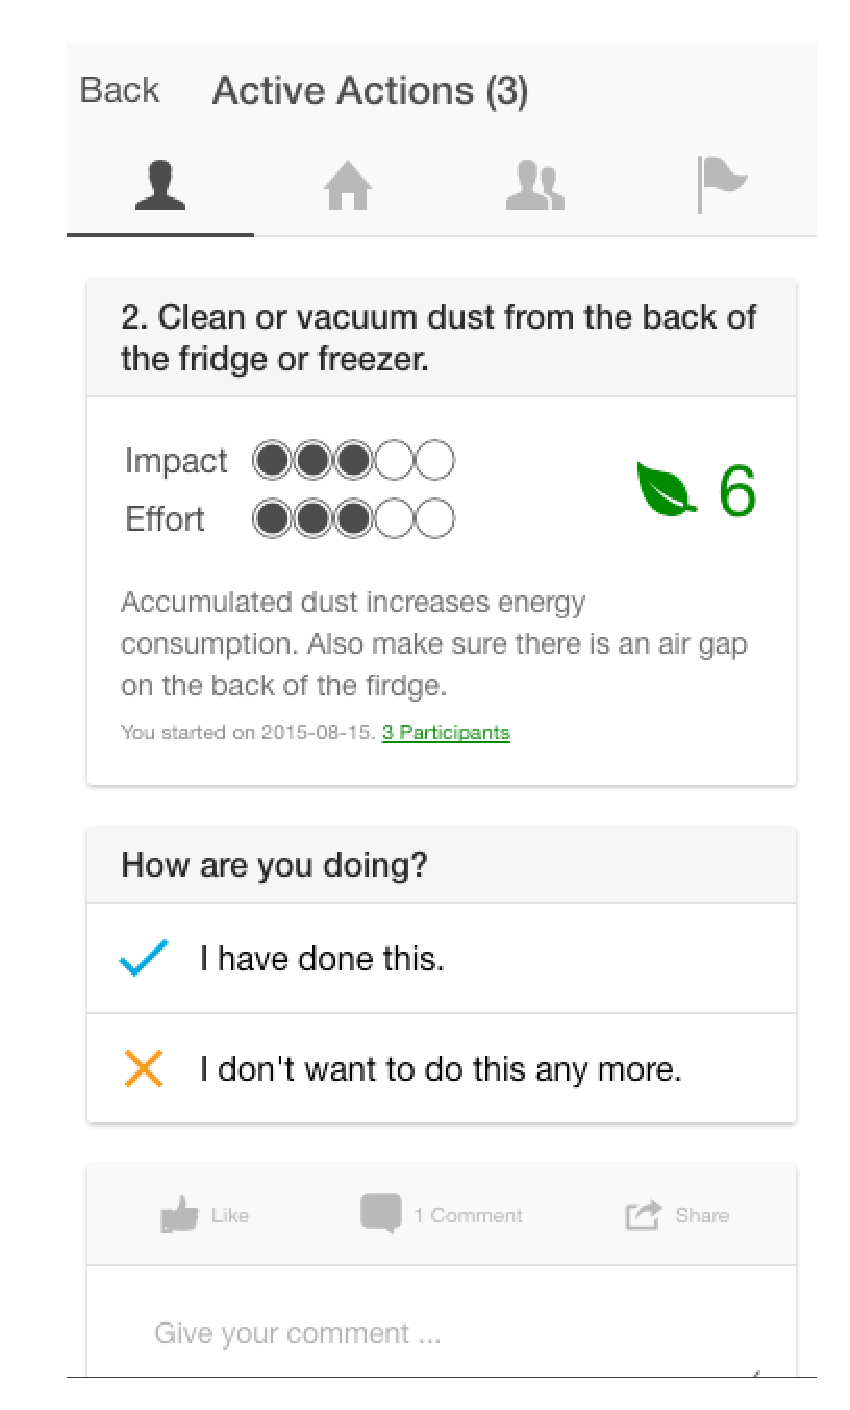
\includegraphics[width=0.33\linewidth]{img/action_details}
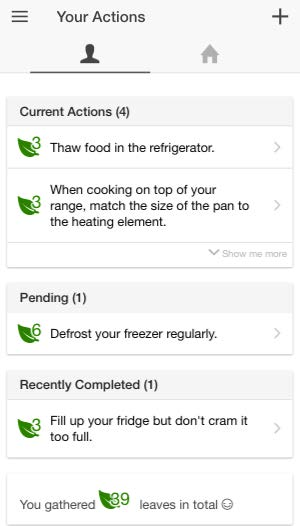
\includegraphics[width=0.33\linewidth]{img/action_tab}
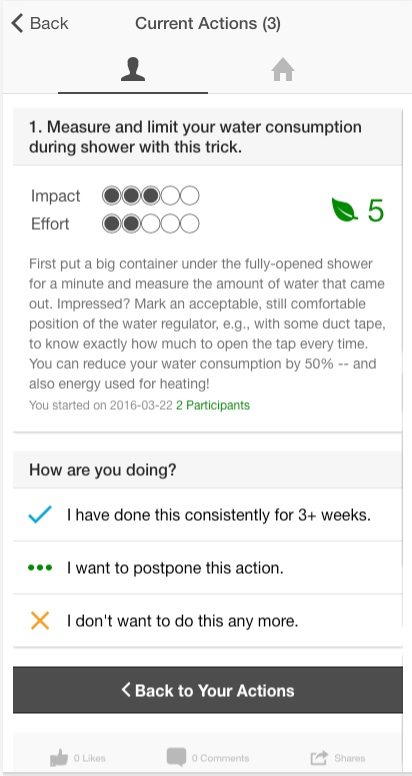
\includegraphics[width=0.307\linewidth]{img/Your_Actions.jpg}
\caption{(1) An action suggestion; (2) User actions tab; (3) An action in progress
}
\label{fig:actions}
\end{figure}

The YouPower application also uses a number of other design elements to promote users' motivation and engagement in the behavior change process. In principle, the focus is placed on providing supports for relatedness, competence and autonomy, promoting pro-environmental and altruistic values, and making one's energy conservation actions and commitments more publicly observable. 

\begin{figure}[t!]
      \begin{center}
        \begin{minipage}[t!]{0.4\linewidth}
	       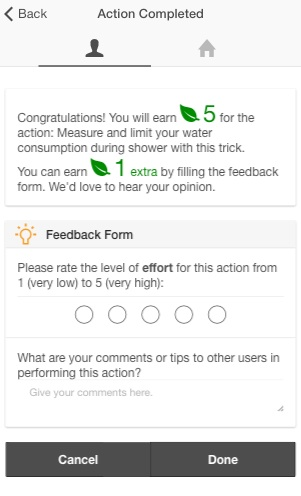
\includegraphics[width=1\linewidth]{img/action_completed.jpg}
           \vspace{2.75cm}
        \end{minipage}
        %\hfill 
        \begin{minipage}[t!]{0.4\linewidth}    
         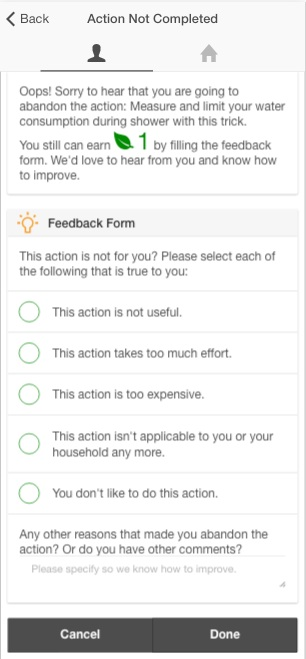
\includegraphics[width=1\linewidth]{img/action_not_completed.jpg}    
        \end{minipage}
      \end{center}
      \caption{Feedback form when a user (1) completes, or (2) abandons an action}\label{fig:form}
\end{figure}

\begin{itemize}
\item Each action has points (displayed as \textit{Green Leaves}) associated to the effort and impact score of that action. If a user completes an action, the user is awarded with leaves.
\item A user can like (with a \textit{Like} button) and comment on the actions (which are visible to all users). After a user completes or abandons an action, the user is asked to provide feedback (to the YouPower team). Figure \ref{fig:form} shows examples. The user is awarded with leaves if he/she gives comments and feedback (1 leaf each). 
\item The application encourages users to take small steps and gives them positive performance feedback. For example, when a user is taking up many actions, the application can prompt that \textit{You already have $x$ actions in progress. You can add more actions after some of those are completed. Keep on! You are doing great.} 
\item A user can signup and login YouPower with a Facebook account. If so, the user can ``share'' an action on Facebook. Figure \ref{fig:share} shows an example. 
\item The users are presented with the information about how many users have been taking an action (including Facebook friends when logged in through Facebook). 
\item A user can configure a personal profile and household profile.
\item A user can add members to his/her household; Figure \ref{fig:house}-(1). If so, the user can see the actions of household members; Figure \ref{fig:house}-(2), and add the actions to his/her own action list.
\item A user can send friends Email invitations to join YouPower (Figure \ref{fig:invite}).
\end{itemize}

\begin{figure}
\centering
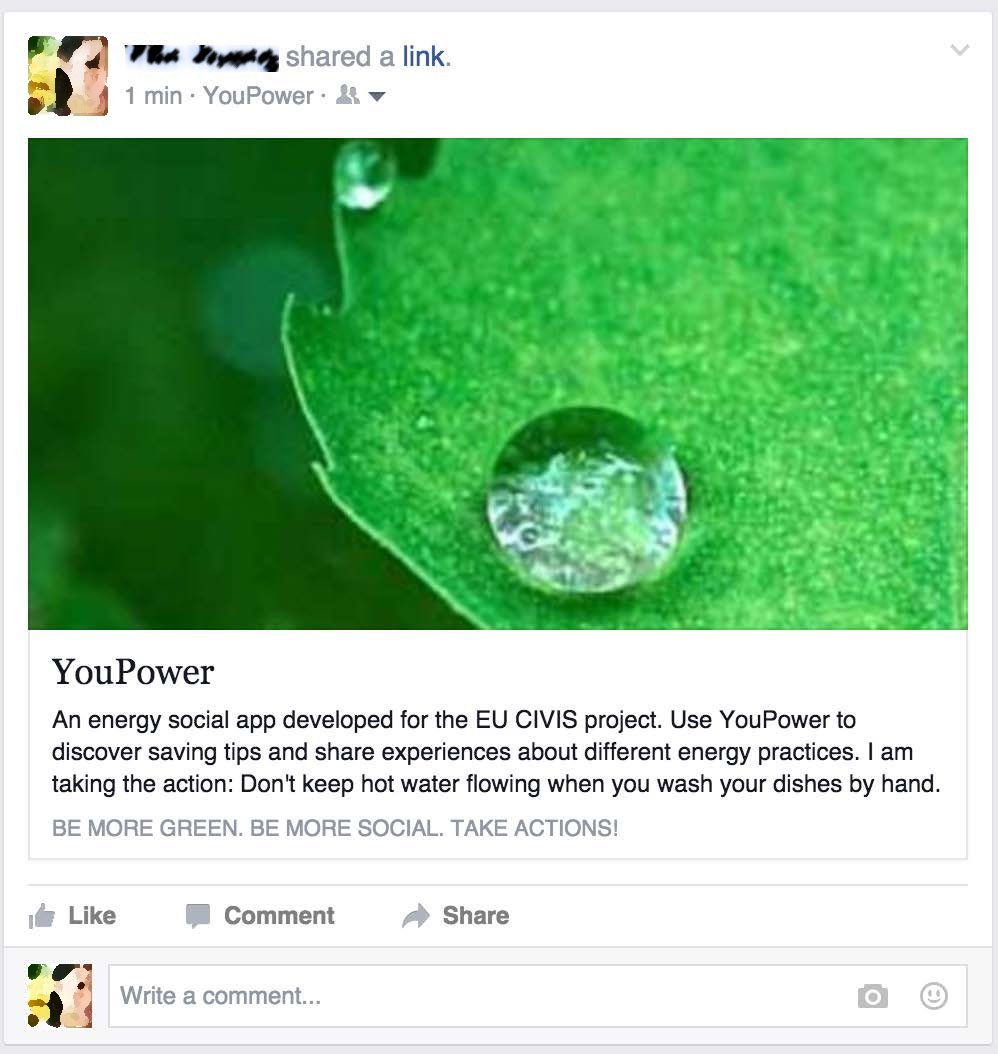
\includegraphics[width=0.62\linewidth]{img/share}
\caption{Facebook share of a YouPower action}
\label{fig:share}
\end{figure}

\begin{figure}[t!]
      \begin{center}
        \begin{minipage}[t!]{0.4\linewidth}
	       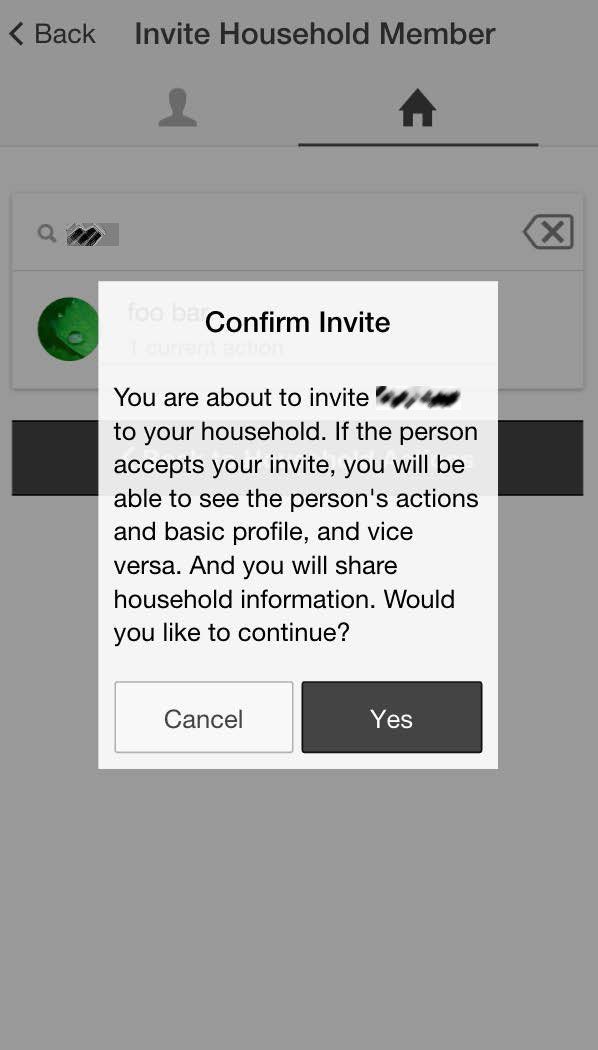
\includegraphics[width=1\linewidth]{img/house1.jpg}
        \end{minipage}
        %\hfill 
        \begin{minipage}[t!]{0.4\linewidth}    
         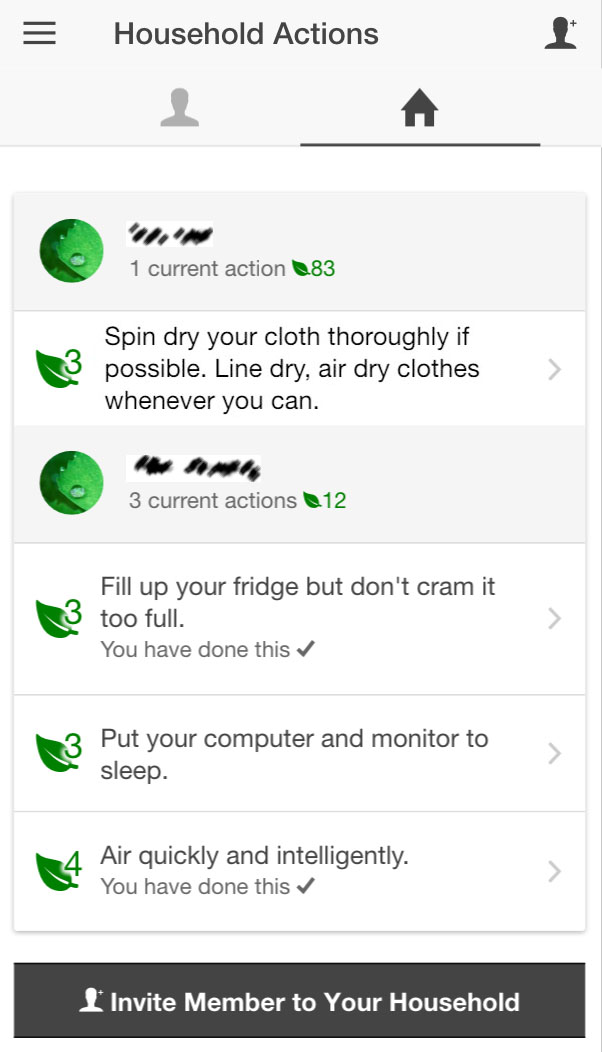
\includegraphics[width=1\linewidth]{img/house2.jpg}    
        \end{minipage}
      \end{center}
      \caption{(1) Invite household member; (2) Household member actions}\label{fig:house}
\end{figure}

\begin{figure}[t!]
      \begin{center}
        \begin{minipage}[t!]{0.34\linewidth}
	       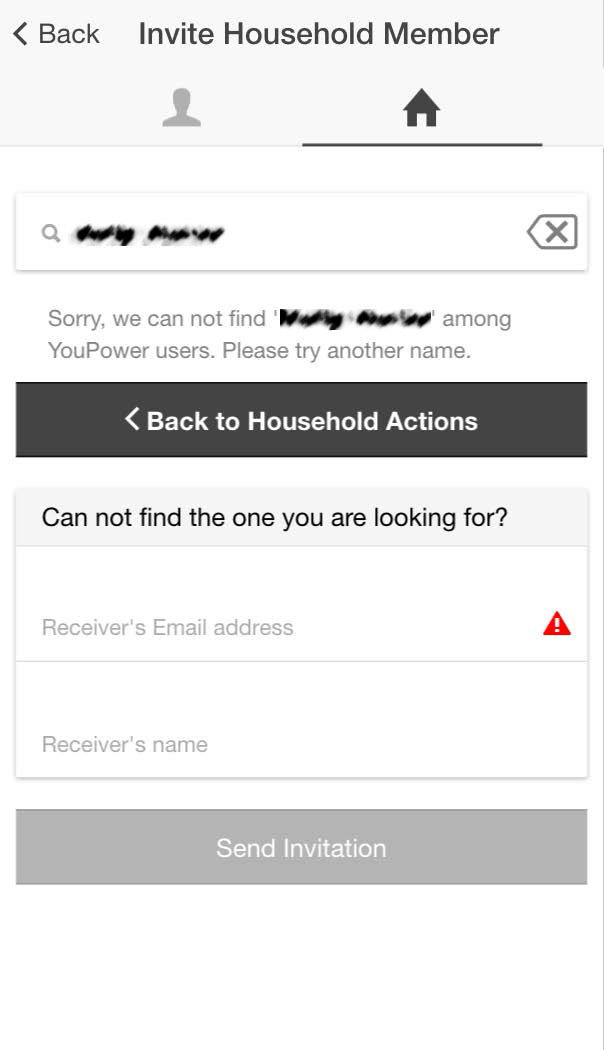
\includegraphics[width=1\linewidth]{img/invite1.jpg}
        \end{minipage}
        %\hfill 
        \begin{minipage}[t!]{0.65\linewidth}    
         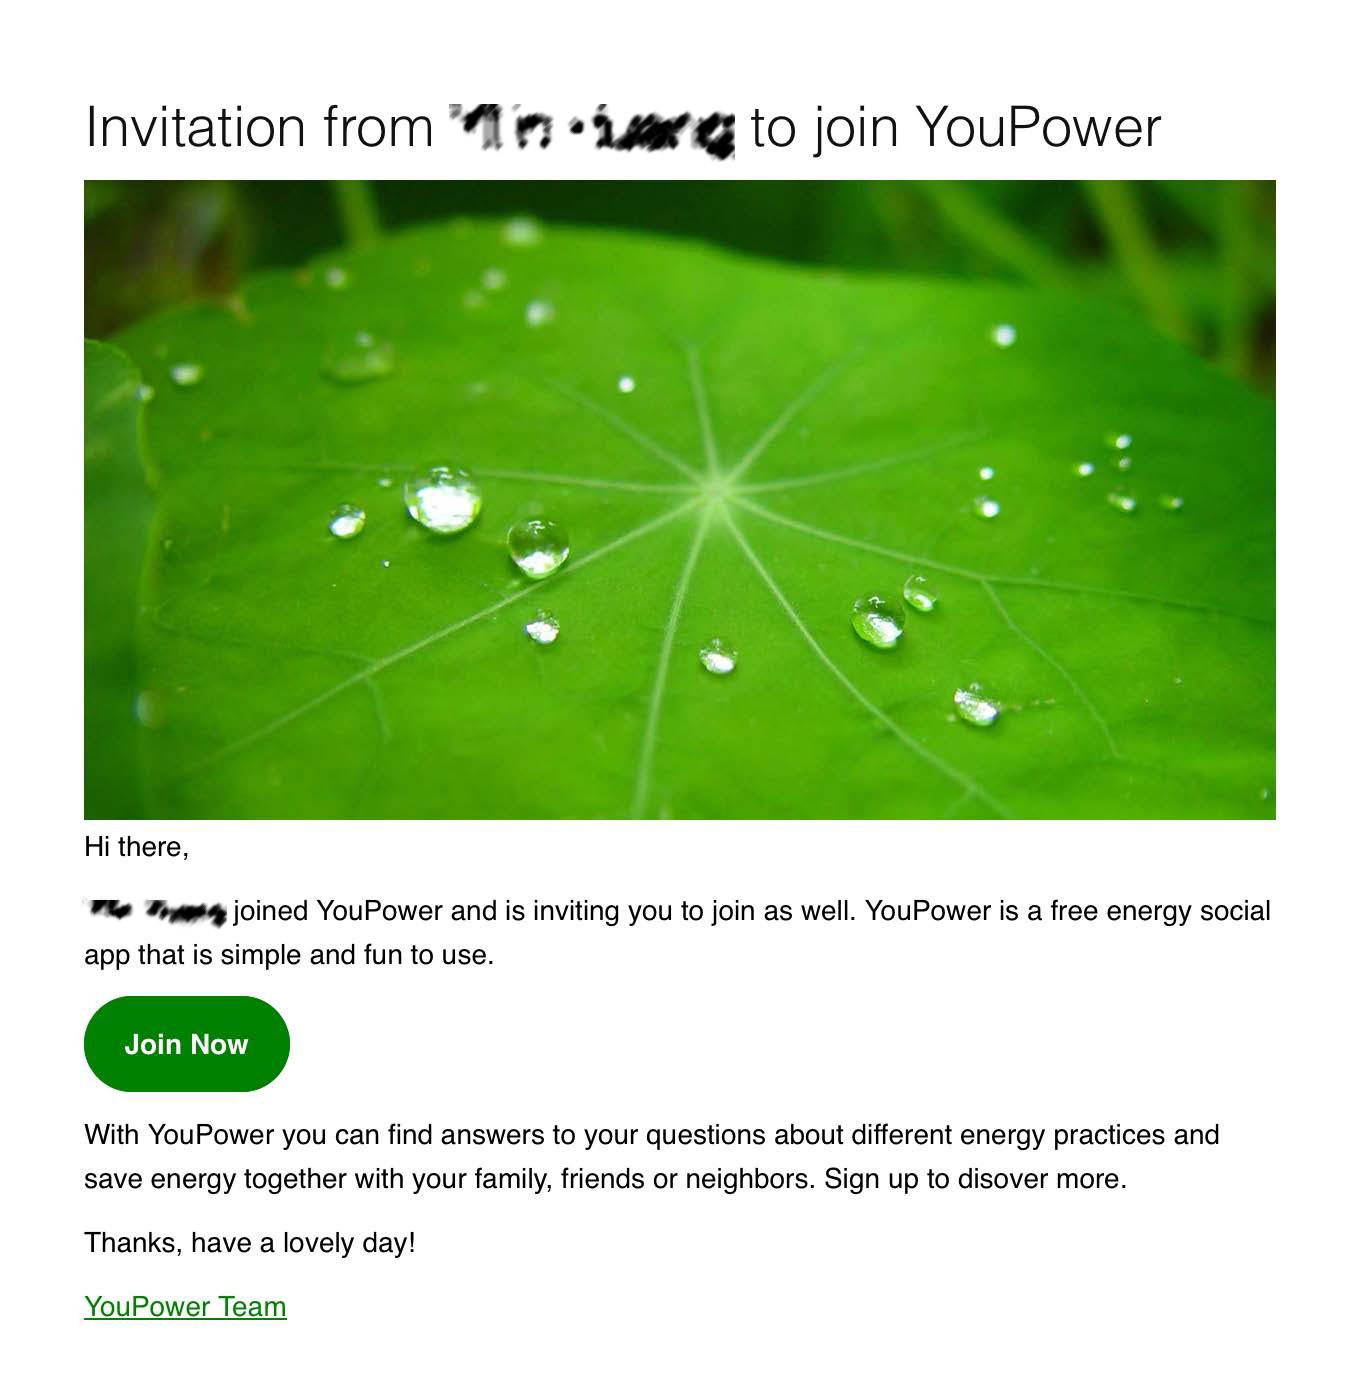
\includegraphics[width=1\linewidth]{img/invite2.jpg}    
        \end{minipage}
      \end{center}
      \caption{Send Email invitation to join YouPower }\label{fig:invite}
\end{figure}

The intention of the design (besides those already mentioned) can be highlighted as follows. For the options of choosing actions, see e.g. Figure \ref{fig:actions}-(1) and Figure \ref{fig:actions}-(3), first person narrative (e.g. \textit{I don't want to do this}) is used to create a personal micro-environment for the user \citep{Crumlish2009} to have a moment of self-reflection on his/her own energy conservation actions, e.g. \textit{Does this action make sense to me (or my household)? Am I indeed doing this? Do I want to do this?} By doing so, the user can identify whether an action is feasible in her/his own context, and whether there is an attitude-behavior gap present with regard to that particular action, and if so should he/she (and would he/she like to) change it; see e.g. Figure \ref{fig:actions}-(1) and Figure \ref{fig:actions}-(3). 

For the framing of the actions, feedback forms, and other parts of the YouPower interface such as prompt messages, \textit{we} is used referring to the YouPower team, and \textit{you} to address the user (see e.g. Figure \ref{fig:form}). This ``talk like a person'' technique (communicating with the participants in a human voice) is often used in designing social interfaces to adopt a conversational tone which provides an opportunity for users to enter into a dialog with YouPower, creating a non-solipsistic and receptive state of mind \citep{Crumlish2009}. ``Self-deprecating message'' are used e.g. when a user abandons an action (``Oops! Sorry to hear that you are going to abandon the action''), and when there is no results for a search (``We can not find `foo bar' among YouPower Users''). Error messages and alike should always put the blame squarely on the shoulders of the product's owners and not on those of the users \citep{Crumlish2009}. 

Users can freely choose whether (and when) to take an action and possibly reschedule and repeat the action according to their own needs and interests. After all, users are experts of their own reality. This makes individual actions and the series of actions suitable in the context of the user's everyday household practices so that he/she can adapt and follow the process of action-taking at a pace that suits his/her situations. Users have free choices of actions as revocable self-commitments, as well as whether to give feedback and invite household members or new users, etc. This facilitates the sense of autonomy which enhances and maintains motivation. Users' choices, e.g. the commitment to an action, the completion or cancellation of an action, together with the other user inputs such as comments and feedback, etc., make a good data source for further research and personalization of the content. 

With an in-context email form (see e.g. Figure \ref{fig:invite}), a user can send an invitation to a friend asking to join YouPower. The benefits of joining and participating in YouPower are clearly articulated to the recipient in the email with a ``call to action'' button \citep{Crumlish2009}. A user can also send household member invitations and act upon them after receipt. By creating households and adding household members, users can have an overview of the household actions. Household energy conservation needs joint efforts, and household members can share the responsibility. The social features such as \textit{Like, Comment, Share, Invite} add social dynamics among users who can share and discuss their experiences and reflections with others. 

\subsubsection{Housing Cooperatives}

\paragraph{Aim and target group}

The housing cooperative part of the application is used by housing cooperatives in \textit{Hammarby Sj{\"o}stad}, Stockholm Test Site. This part provides features for building level energy information and actions. 

 All apartment owners in Sweden have to be members of a housing cooperative that owns the building. A board is elected among the members and the board is in charge of the cooperative's finances and maintenance of the building. This work may include deciding on energy contracts, making sure energy systems are maintained and proposing investments in more energy efficient technologies. People in the board are volunteers who may have no previous knowledge of energy or building management. Hence, the housing cooperative part of the app aims to support board members in energy management work and, more specifically, in taking energy reduction actions.

In Hammarby Sj{\"o}stad, some of the housing cooperatives have an appointed energy manager in the board who is responsible for the energy work. This role, no matter if it is explicitly named energy manager or if it is an implicitly shared responsibility among several board members, is the primary target for the housing cooperative part of the app. The app can also be used by other housing cooperative members who are interested in following the energy work of the cooperative. A third type of user is energy or building management companies working with housing cooperatives. All information in the app is visible for all these user groups and shared between housing cooperatives. This openness of energy data is key to facilitating the users in sharing experiences relevant for taking energy reduction actions.

\paragraph{Linking energy data to energy reduction actions}

One of the main housing cooperative features of the app is that it allows for linking energy data with energy reduction actions taken, which makes it possible to follow up on the impact of energy actions (see Figure \ref{fig:Figure201_Actions}). The energy use is divided into heating and hot water (from district heating) and facilities electricity and the user can switch between these views in the energy use graph (see Figure \ref{fig:Figure201_Actions}, left). The user can also choose between viewing energy use per month or per year. This provides enough level of detail to show overall changes in energy use. Since the energy data is shared between cooperatives there may also be privacy concerns related to opening up data of higher granularity to people outside of the own cooperative. 

\begin{figure}
	\centering
	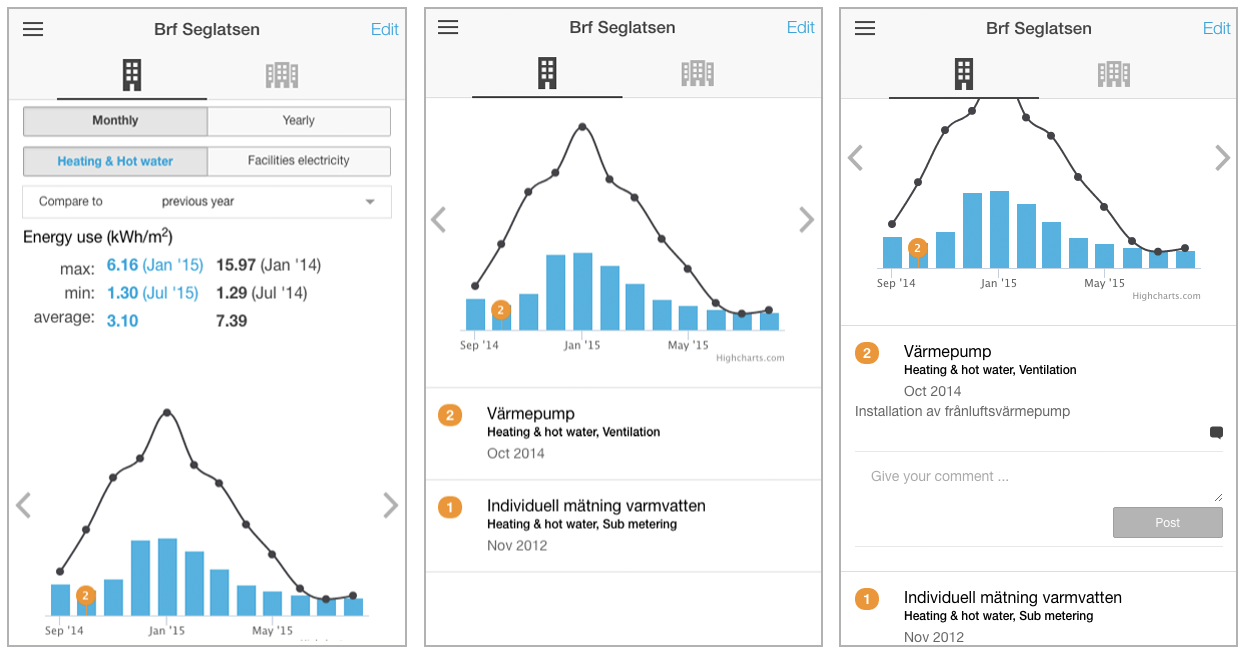
\includegraphics[width=0.98\linewidth]{img/Figure201_Actions.png}
	\caption{Energy use graph where the blue bars show the current year's energy use and the black line shows the previous year's energy use. Energy reduction actions taken are mapped to the graph and listed below.}
	\label{fig:Figure201_Actions}
\end{figure}

Users with editing rights, typically energy managers or other boards members, can in the app add energy reduction actions that the cooperative has taken, including information about:
\begin{itemize}
\item Title of the action.
\item Type of energy action (e.g. heating optimisation, action affecting the ventilation or action to make lighting more efficient). The action types are in the form of tags (more than one can be added to each action), which makes it possible to add functionality for filtering or searching for specific actions.
\item Month and year the action was taken or completed.
\item Cost for taking the action.
\item Additional details about the action.
\end{itemize}

Energy or building management companies that work with a cooperative can also get editing rights and add energy reduction actions they take on behalf of the cooperative. Added actions appear in the energy use graph at the month when each action was taken and all actions are listed below the graph. When clicking on an action in the list, the action is expanded and the details of the action are shown.

To make the impact of energy reduction actions visible, the user can choose to compare the energy use of the viewed months to the energy use of the same months the previous year. This can be used for example when a housing cooperative wants to explore what energy reduction actions to take in the future by looking at the actions taken by other cooperatives and what the effects were in relation to costs.

\paragraph{Comparing housing cooperatives}

A user can see all cooperatives who are using the app in a map view or list view (see Figure~\ref{fig:Figure202_Housing_cooperatives_comparison}). To facilitate comparison between cooperatives the icons in the map and list are colour coded based on each cooperative's energy performance, i.e. the energy use per square meter heated area (kWh/m$^2$). It uses a scale from red to green, where a red colour indicates a poor energy performance (i.e. high energy use) and a green colour indicates good energy performance (i.e. low energy use). The energy performance scale is calculated in a similar way as for the Swedish energy declaration for buildings\footnote{\url{http://www.boverket.se/sv/byggande/energideklaration/energideklarationens-innehall-och-sammanfattning/sammanfattningen-med-energiklasser/energiklasser-fran-ag/}}  but it is calibrated to only include measured energy use for heating and hot water, which is the greatest part of the energy use. In the Swedish energy declarations, facilities electricity is also added but that often requires estimations of different factors to make the number comparable.

\begin{figure}
	\centering
	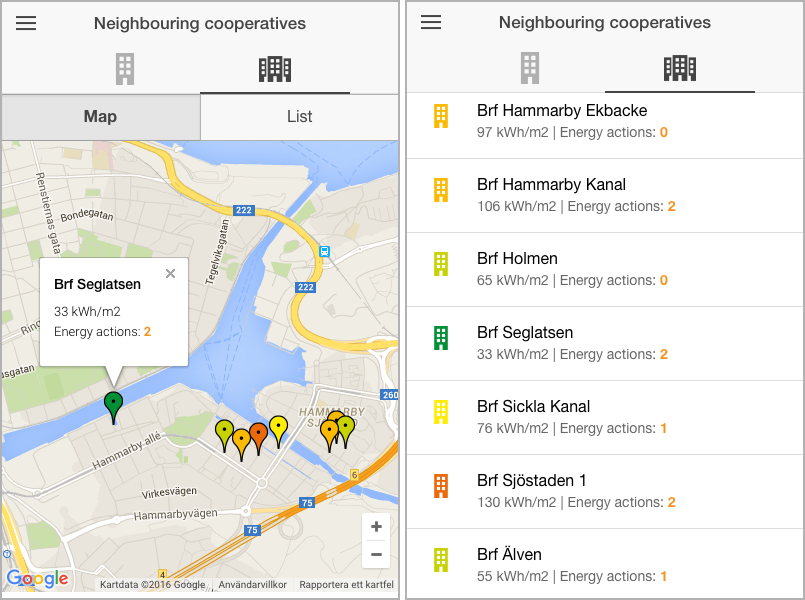
\includegraphics[width=0.9\linewidth]{img/Figure202_Housing_cooperatives_comparison.png}
	\caption{Map and list view of participating housing cooperatives. The energy performance of the cooperatives is indicated by colour and in numbers.}
	\label{fig:Figure202_Housing_cooperatives_comparison}
\end{figure}


For each cooperative in the list or on the map, the user can also see the energy performance as a number (kWh/m$^2$) and the number of energy reduction actions taken. The number of actions is important to display to make energy reduction efforts of housing cooperatives with a high energy performance (e.g. due to poor construction of the building) visible. 

The energy managers in the project stressed that it is important to know what type of housing cooperative you are comparing your own to, in order to understand what any differences in energy performance may depend on and which of their experiences could be relevant for the own cooperative. Therefore, the app provides the following information about each cooperative (see Figure \ref{fig:Figure203_cooperative_info}):
\begin{itemize}
\item Number of apartments in the cooperative.
\item The cooperative's heated area ($m^2$).
\item The building's construction year.
\item Type of ventilation (e.g. with or without heat recovery).
\end{itemize}

\begin{figure}
	\centering
	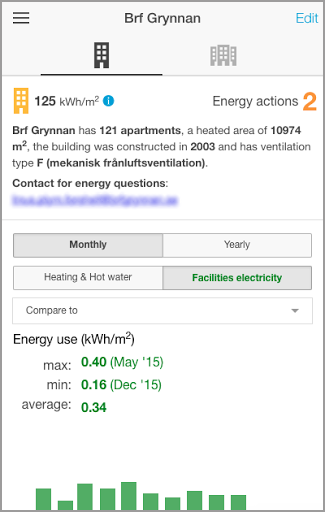
\includegraphics[width=0.4\linewidth]{img/Figure203_cooperative_info.png}
	\caption{Information about the housing cooperative that is important for understanding the energy performance and actions taken is displayed in the top of the page.}
	\label{fig:Figure203_cooperative_info}
\end{figure}

While the energy performance provides a comparison of the current situation, there is also a feature for comparing a cooperative's energy use over time to the neighbourhood average (see Figure \ref{fig:Figure204_Neighbourhood_average}). In the energy use graph for each cooperative, divided into heating and hot water and facilities electricity, the user can display the average energy use of the other cooperatives using the app. In that way, the user can get an idea of how a cooperative's energy use has changed over time in relation to other cooperatives. To make the energy use comparable between cooperatives, the energy in the graphs is (in the same ways as the energy performance) displayed as energy use divided by heated area (kWh/m$^2$).

\begin{figure}
	\centering
	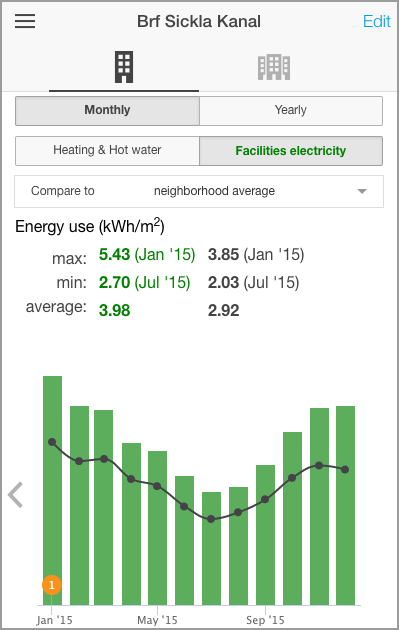
\includegraphics[width=0.4\linewidth]{img/Figure204_Neighbourhood_average.png}
	\caption{The green bars show the monthly facilities electricity use of the housing cooperative and the black line shows the average facilities electricity use for all housing cooperatives using the app.}
	\label{fig:Figure204_Neighbourhood_average}
\end{figure}

\paragraph{Sharing experiences}

The details about each energy action taken by a cooperative, together with the effects on the energy use, provides information that could support other cooperatives in learning more about which energy reduction actions are effective. However, a cooperative that is interested in taking an action may want more information than what is provided by the person adding the action, e.g. regarding how to take an action, which contractor was used for an investment or how to get buy-in from the cooperative members. The app supports this through a commenting function for each action added, where users can post questions related to the action. The cooperatives can also choose to add an email address to their energy contact person, which is visible on the cooperatives app page, to allow for direct contact.

Sharing of experiences of course also happens outside of the digital world, e.g. during housing cooperative board meetings or meetings with the local energy network in Hammarby Sj{\"o}stad. The app is aiming to support discussions and knowledge exchange also in such situations, and it should be easy for someone who wants to demonstrate the impact of an energy investment to just take out the smart phone and show the visualization. Consequently, the mobile screen format is an important part of the design.

\subsubsection{Energy awareness at individual and collective levels}\label{sec:energydata}

This part of the application is designed and developed to enable an informed approach to ``fair energy use'' by making people aware of their
energy behaviors in individual and collective terms. Indeed, it includes means for users to visualize in an easily
understandable and actionable way a specific set of energy measurements, simple analytics and a time-of-use signal.

The access point for this part of the app is the ``Energy Data'' navigation tab (Figure \ref{fig:tab}). This tab gives access to an
overview of the various functionalities and visualizations of specific information: ``Energy Meteo'', Visualization of consumption and production data (real time and historical),
``Comparisons'' data.

There are three main categories of information provided through this part of the app:
\begin{itemize}
 \item Time of use signal
 \item Visualization of real time and historical data (individual level)
 \item Comparative visualizations (collective level)
\end{itemize}

\begin{figure}[htb]
\centering
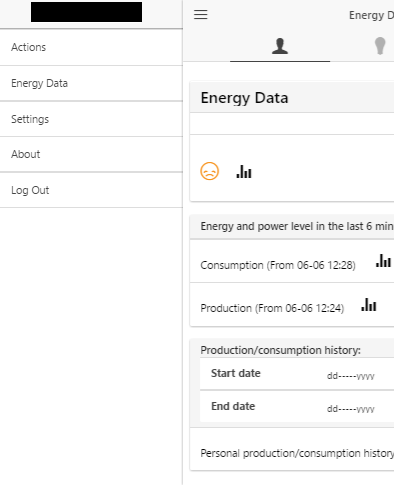
\includegraphics[width=0.33\linewidth]{img/trentinooverview_tab3.png}
% 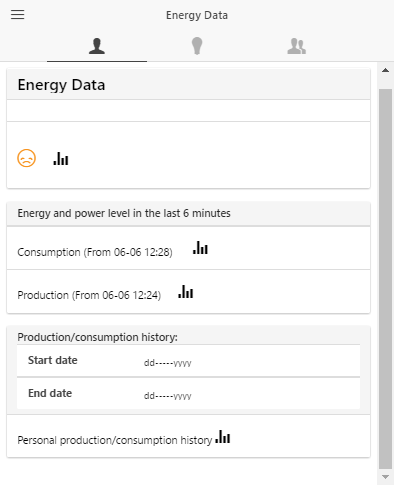
\includegraphics[width=0.33\linewidth]{img/trentinooverview3.png}
% 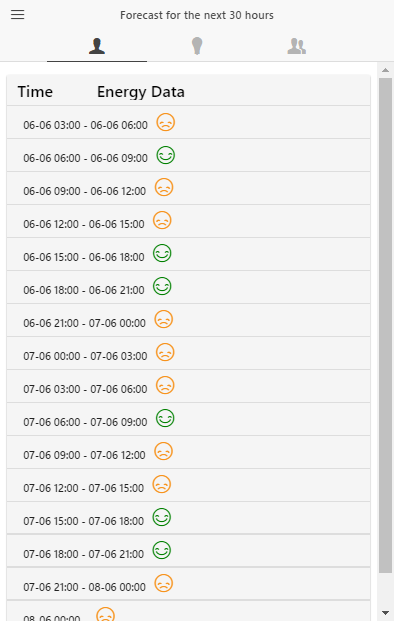
\includegraphics[width=0.307\linewidth]{img/touprediction.png}
\caption{Navigation tab with access to the feature for energy awareness: ``Energy Data''}\label{fig:tab}
\end{figure}

Although the direct impact of these kind of information can be debated -- reported reductions ranging from 2\% to 20+\% \citep{eea_report} and the fact the their medium and
long-term implications received some criticisms (with particular regards to normative `eco-feedback'~\citep{Strengers2012,Cakici2014}), this part of the app is in-line with the needs emerged from
the pilot sites and the project activities\footnote{Requirements analyzed as reported in Deliverable 3.1. Design concept validated as reported in Deliverable 3.2.}.
It also addresses the fact that improvements of dwellers' energy awareness remain a necessary condition towards the long-term adoption of more sustainable behaviors,
although not sufficient alone. Indeed, this part of the app has been designed with broader processes of social change
in mind\footnote{For further details, see the User Story ``Energy Garden'' included in Deliverable 1.3.}. Therefore, ``energy awareness'' should be considered as instrumental to
well defined individual and collective efforts. 



\paragraph{``Energy Meteo'': the Time-of-Use (ToU) signal} is designed to leverage load elasticity for maximizing self-consumption, with the twofold effect of optimizing usage of locally-installed RESs and minimizing dependency from energy markets. This means that electric loads shall be shifted to periods of time characterized by high local production from renewable energy sources.
It provide users with a clear indication of the actual status of the local grid: \textit{green smilies} signal slots when local production exceeds demand; \textit{orange smilies} highlight slots
when demand exceeds local production\footnote{See Deliverable 4.2 \textbf{[NB: VERIFY!!]}, for more details on the technical design and implementation of the predictive model of the ToU signal.}.

\begin{figure}[htb]
      \begin{center}
        \begin{minipage}[htb]{0.33\linewidth}    
         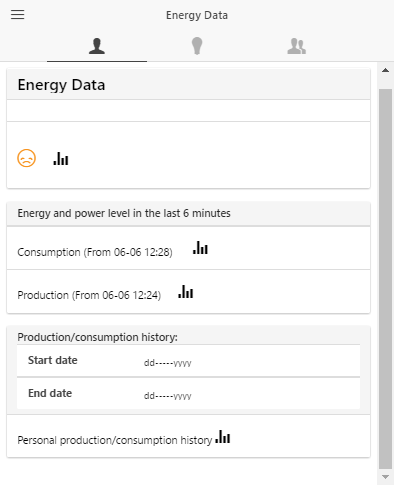
\includegraphics[width=1\linewidth]{img/trentinooverview3.png}   
        \end{minipage}
% 	\hfill 
        \begin{minipage}[htb]{0.33\linewidth}    
         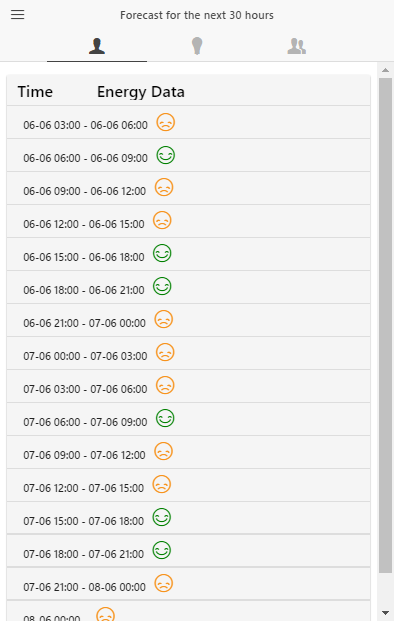
\includegraphics[width=1\linewidth]{img/touprediction.png}   
        \end{minipage}
      \end{center}
      \caption{(1) ``Energy Data'' main screen: overview of the various functionalities and easy access to visualization of specific information;
(2) ToU signals with a 30-hours forecast, divided by 3-hours slots.}\label{fig:overview-tou}
\end{figure}

The ToU signal is provided in two distinct ways:
\begin{description}
 \item[Current.] It is available on the main screen (Figure \ref{fig:overview-tou}-1) and it indicates whether \textit{present} moment is a good or bad moment to consume locally produced electricity.
 \item[Forecast.] It is available by clicking on ``Energy Meteo'' field and it provides a detailed overview of the local grid conditions, forecasted in 3-hours time-slots, for the forthcoming 30 hours (Figure \ref{fig:overview-tou}-2). A new forecast is generated every 24 hours.
\end{description}



\paragraph{Visualization of consumption and production (real time)} is designed to inform users about their (near to) real time electric consumption and (where available) production data.
\begin{figure}[htb]
      \begin{center}
        \begin{minipage}[htb]{0.33\linewidth}    
         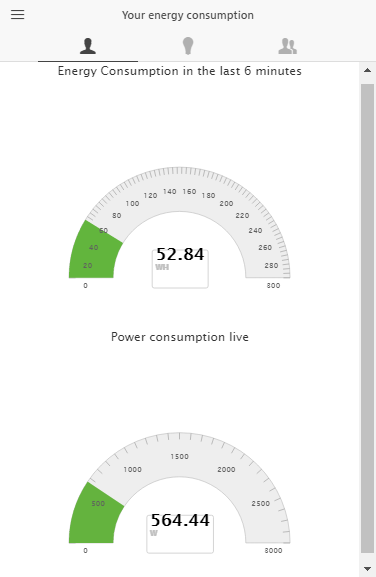
\includegraphics[width=1\linewidth]{img/visual_consumption.png}  
        \end{minipage}
% 	\hfill 
        \begin{minipage}[htb]{0.33\linewidth}    
         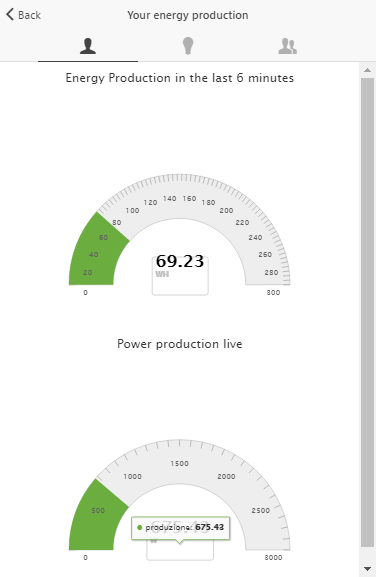
\includegraphics[width=1\linewidth]{img/visual_production.png}  
        \end{minipage}
      \end{center}
    \caption{(1) Energy and Power meters for household's electric consumption measurements; (2) Energy and Power meters for household's electric production measurements.
}
\label{fig:viz_rt}
\end{figure}

Users can access these information from the ``Energy Data'' main screen and either visualize the household's electric consumption (Figure \ref{fig:viz_rt}-1) or
household's electric production (Figure \ref{fig:viz_rt}-2).
These visualizations provide meters for:
\begin{description}
 \item[Energy.] It is accounted for the most recent 6-10 minutes monitored.
 \item[Power.] It provides instant measurement\footnote{For technical reasons and depending on several environmental factors (\textit{e.g.} households connectivity for transfer of monitored data) there may be up to approximately 2 minutes delay of the actual power measured and the data displayed through You Power.}.
\end{description}



\paragraph{Visualization of historical data} is designed to provide users with a broader temporal overview on their energy habits.
\begin{figure}[htb]
      \begin{center}
        \begin{minipage}[htb]{0.33\linewidth}    
         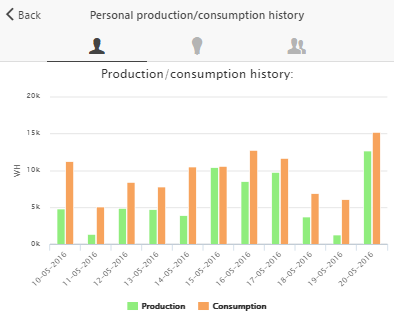
\includegraphics[width=1\linewidth]{img/historicalcomparison_prodcons.png}
        \end{minipage}
% 	\hfill 
        \begin{minipage}[htb]{0.33\linewidth}    
         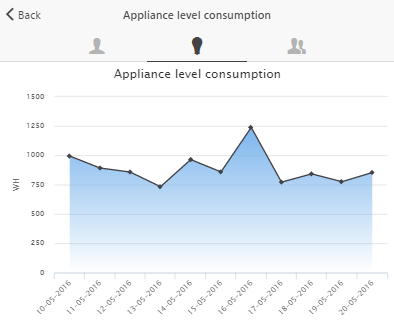
\includegraphics[width=1\linewidth]{img/applianceconsumption.png}
        \end{minipage}
      \end{center}
      \caption{(1) Household overview of electric energy consumption and production, for the chosen data range; (2) Consumption patterns for the chosen data range at appliance level.
}
\label{fig:viz_hist}
\end{figure}

Information about historical data are available both for household and appliance levels:
\begin{description}
 \item[Household.] It provides a daily overview of the overall electric energy consumption and production for the chosen data range. This shall give a basis for dwellers to understand and improve their self-consumption.
 \item[Appliance.] It provides a detailed view of the consumption patterns for the selected appliance. Visualized appliances are the ones equipped with smart plugs. 
\end{description}
Selection of data ranges are mandatory for these visualizations. They must be set by users at two different places: in the ``Energy Data'' main screen for the \textit{Household} category;
in the `light-bulb' sub-view for the \textit{Appliance} one, which is accessible from the top level bar.


\paragraph{Comparisons} are designed to provide users with reference information about energy performances or behaviors in relation to the neighborhoods.
\begin{figure}[htb]
      \begin{center}
        \begin{minipage}[htb]{0.33\linewidth}    
         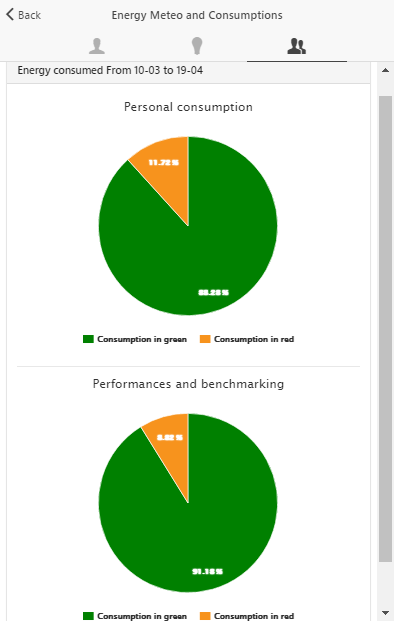
\includegraphics[width=1\linewidth]{img/touperformancechart_indivcoll.png}
        \end{minipage}
% 	\hfill 
         \begin{minipage}[htb]{0.33\linewidth}    
         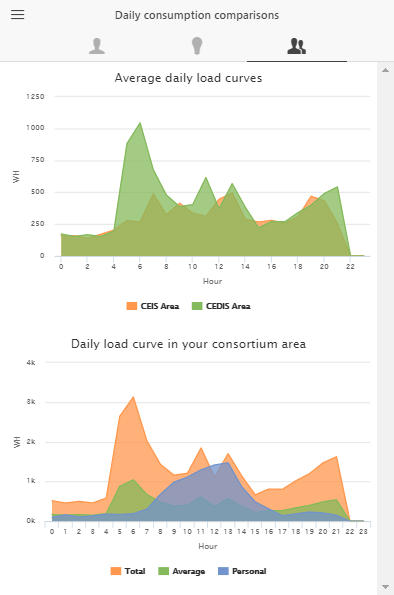
\includegraphics[width=1\linewidth]{img/benchmark.png}
        \end{minipage}
      \end{center}
      \caption{(1) Compares individual consumption with community one with regards to the distribution between delivered ToU signals; (2) Compares: (a) Consumption level between municipalities(test sites), (b), Individual consumption with average and total consumption of household's municipality(test site).
}
\label{fig:comparison}
\end{figure}

\begin{description}
 \item[Consumption distribution on ToU signals] It shows a cumulative and progressive distribution of consumption between the green an red ToU signals.
 On the top part it shows the individual household chart, while on the bottom, the community\footnote{In this case community refers to the registered users who 
 are served by the same Energy cooperative through the same local distribution network.} total distribution. This view is a static one and is progressively updated on a weekly basis. The descriptive label for the chart clearly highlights the reference period considered.
 \item[Consumption profile benchmark] It provides users with a benchmark\footnote{While in principle homogeneous groups of users could be identified to make the comparison more sound, this requires data (household composition, size of dwelling, type and number of appliances preset, thermal isolation \ldots) which are not currently available for the vast majority of the users engaged in the pilot.
 Furthermore, the heterogeneity and limited number of users involved would not allow to form meaningful groups for creating sound averages and benchmarking. For this reason the simple community average is used as a benchmark.} of consumption profile. \textbf{LAST MODULE UNDER DEVELOPMENT - FURTHER DESCRIPTION TO BE ADDED.}
\end{description}
The first feature can be accessed by clicking on the `community' icon, which is symbolized by the two people on the top level bar.
The second feature can be accessed from ``Energy Data'' main screen, by clicking on `comparison' field.

\paragraph{Participatory Budgeting external service} is implemented to accompany users along their efforts and process of changing their energy behaviors.
Particularly, with regards to the collective objective to maximize use of locally produced electricity. A website has been implemented to:
\begin{itemize}
 \item detail the conditions and regulations for the participatory budgeting process;
 \item submit idea proposals for the awarding of the `energy bonus';
 \item update involved users about proposals received;
 \item informed users about the various steps along the evaluation and selection procedures for the awarded proposals. 
\end{itemize}
The website can be reached at \url{https://progettocivis.wordpress.com/}.

\clearpage
%


%Survies and statistics show that despite many users are concerned about their energy use, and interested in reducing energy use and saving energy bill, little of them actually know what to do to achieve the goal. 
%Today, consumers still have a vague understanding of the power grid or what they can do with it. This is however very important, because how consumers understand the smart grid will shape how they feel about it, and in turn determines whether they are ready to use it, and how they use it. 
%
%To this end, it is very important how we present energy information (or information or knowledge of the power grid in general) to the users. 
%
%It is clear that we need to provide them with personalized information. And more importantly, we need to give them actionable information. 
%
%If consumers are given useful feedback on how they use energy, and they are given recommendations on how to improve, they will have the chances to make more informed energy choices. 
%
%This may have chances to yield crowdshifting effect, which simply means large-scale, voluntary behavioral change for social good. 
%
%There are many finer details in how to present users with information and how this could affect user behavior. All these are interesting topics to study. 

The side navigation (nav) is composed of six items, among which the ``Energy Data'' and ``Housing Cooperatives'' are activated respectively when a user authenticated his/her household's account for energy data (production is only for the Italian case) or when a user is a member of a housing cooperative (the Swedish case). Each tab item is associated with at least one view. Figure~\ref{fig:menu} shows an example: the ``Action List'' view of ``Your Actions'' tab with a closed (left) and an open (right) side navigation drawer. 

\begin{table}
\caption{YouPower app navigation structure}\label{tab:app_nav}
\begin{center} \footnotesize 
\begin{tabular}{ l l p{6cm}}
\hline
\textbf{Side Nav Items}  &
\textbf{Tab Items}  &
\textbf{Views}  \\ \hline

Actions & Your Actions & Action List, Action Suggestion, Action Details, Action Completed Form, Action Abandoned Form, etc.\\ 
& Household Actions & Member List, Action List, etc. \\ 
& Community Actions & Community List, Top Action List, Discussions, etc.\\ 
& Achievements & Achievement List (unlocked/locked), etc.\\  \hline

Energy Data  & Household Level  & Current Tarif (Trentino only), Current Consumption, Current Production, Historical Production/Consumption Patterns, Forecasted Tarifs (Trentino only)\\ 
& Appliance Level & Consumption Patterns (for each monitored appliance) \\ 
&  Community Level & Total Community Consumption (last month), Total Community Production (last month), Community Energy Balance, Comparison with Benchmark \\  \hline

Housing Cooperatives & Your Cooperative & Action List, Consumption per Category, Discussions, etc. \\ 
& Cooperatives in Neighborhood&  Action Map, Action List, Discussions, etc. \\  \hline

Donation (Trentino only) & n/a & Campaign Information, Campaign Status \\
\hline

Settings & Preferences & Form \\ 
& Personal Profile & Form \\ 
& Household Profile & Form, Eenergy Data Account \\  \hline

About & Q\&A & Q\&A List \\ 
& Help \& Feedback & Contact, Form\\ 
& Version Update & Version Info\\  \hline
\end{tabular}
\end{center} 
\end{table}

\begin{figure}
\begin{center}
	   \frame{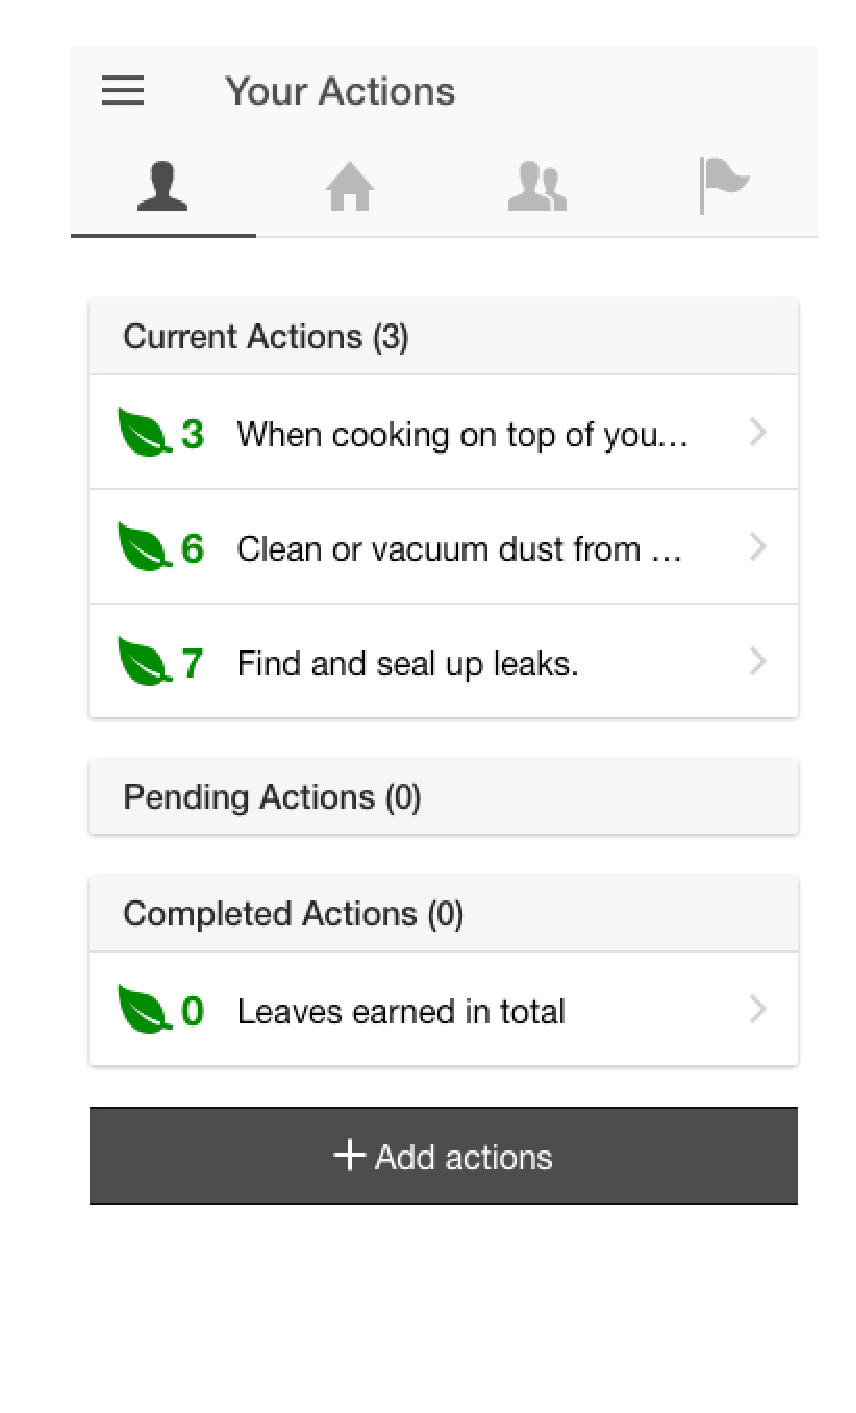
\includegraphics[height=0.55\textheight]{img/your_actions.pdf}}
		 \hfill
	   \frame{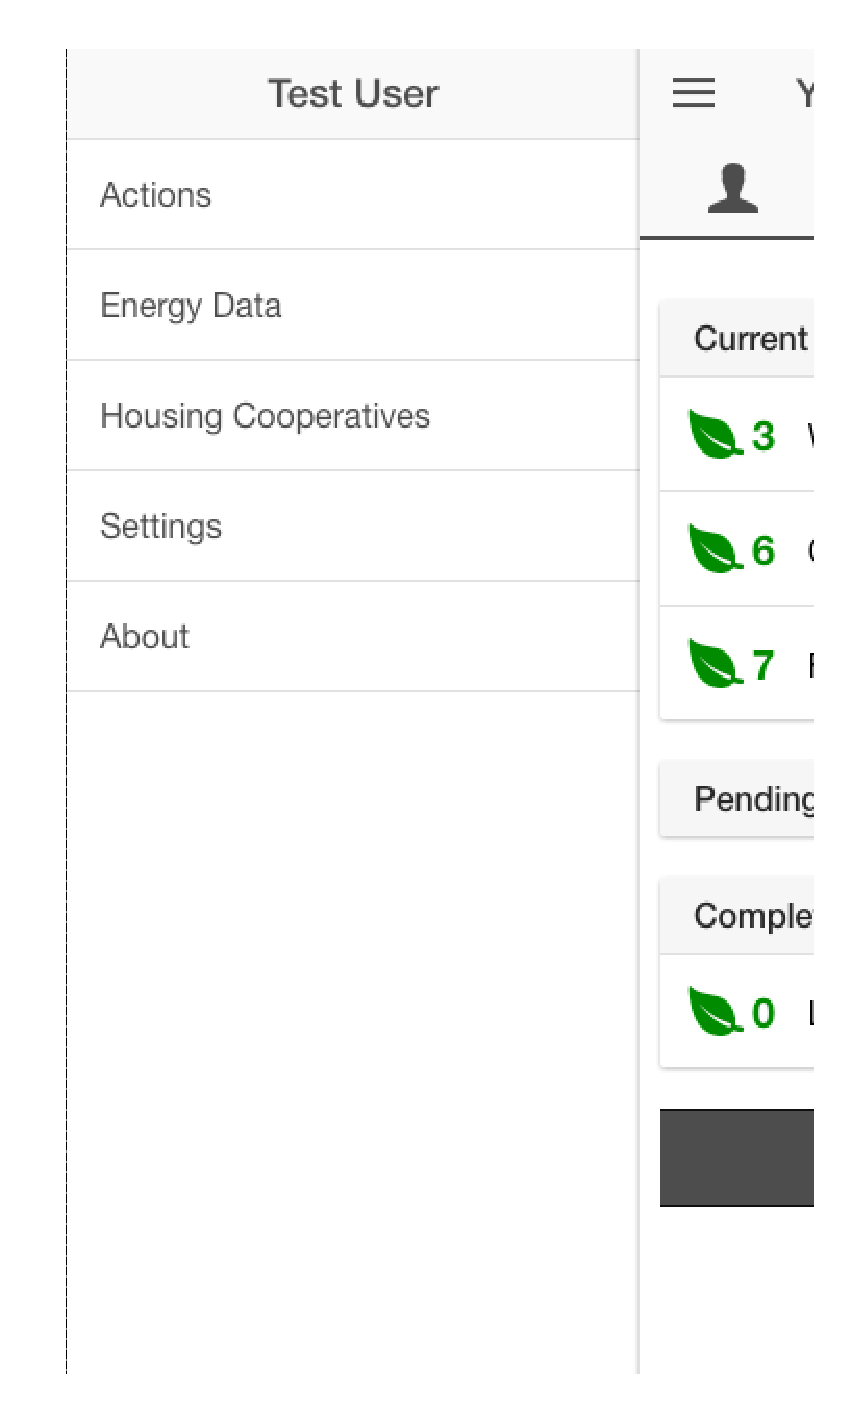
\includegraphics[height=0.55\textheight]{img/menu.pdf}}
	  \caption{``Your Actions'' tab -- ``Action List'' view (left); with an open side nav drawer (right)}\label{fig:menu}
\end{center}
\end{figure} 
The ``Action List'' is the index view of ``Your Actions'' tab. It is also the default view after user login. In this case, when the user presses on one of the ``Current Actions'', the app navigates to the ``Action Details'' view. Figure~\ref{fig:action_details} gives an example. 
% 


\section{CIVIS Platform  Development} 
\label{sec:develop}
 
The development of the CIVIS platform started in May 2015 \citep{Huang2015c} and continued in the third year's WP3 activities. At the time of writing this deliverable (May/Jun 2016), the development is completed with bug fixing and minor updates.
% 
The JavaScript (JS) programming language %\footnote{\url{http://www.crockford.com/javascript/javascript.html}} 
is used for development at both front- and back-ends. 
Figure~\ref{fig:ScreenShot2015-11-09at18} provides an overview of the major technologies used at the front-end and back-end. They are discussed in this section. 
% The platforms and technologies mentioned are all free and open source. 

\begin{figure}[h!]
\centering
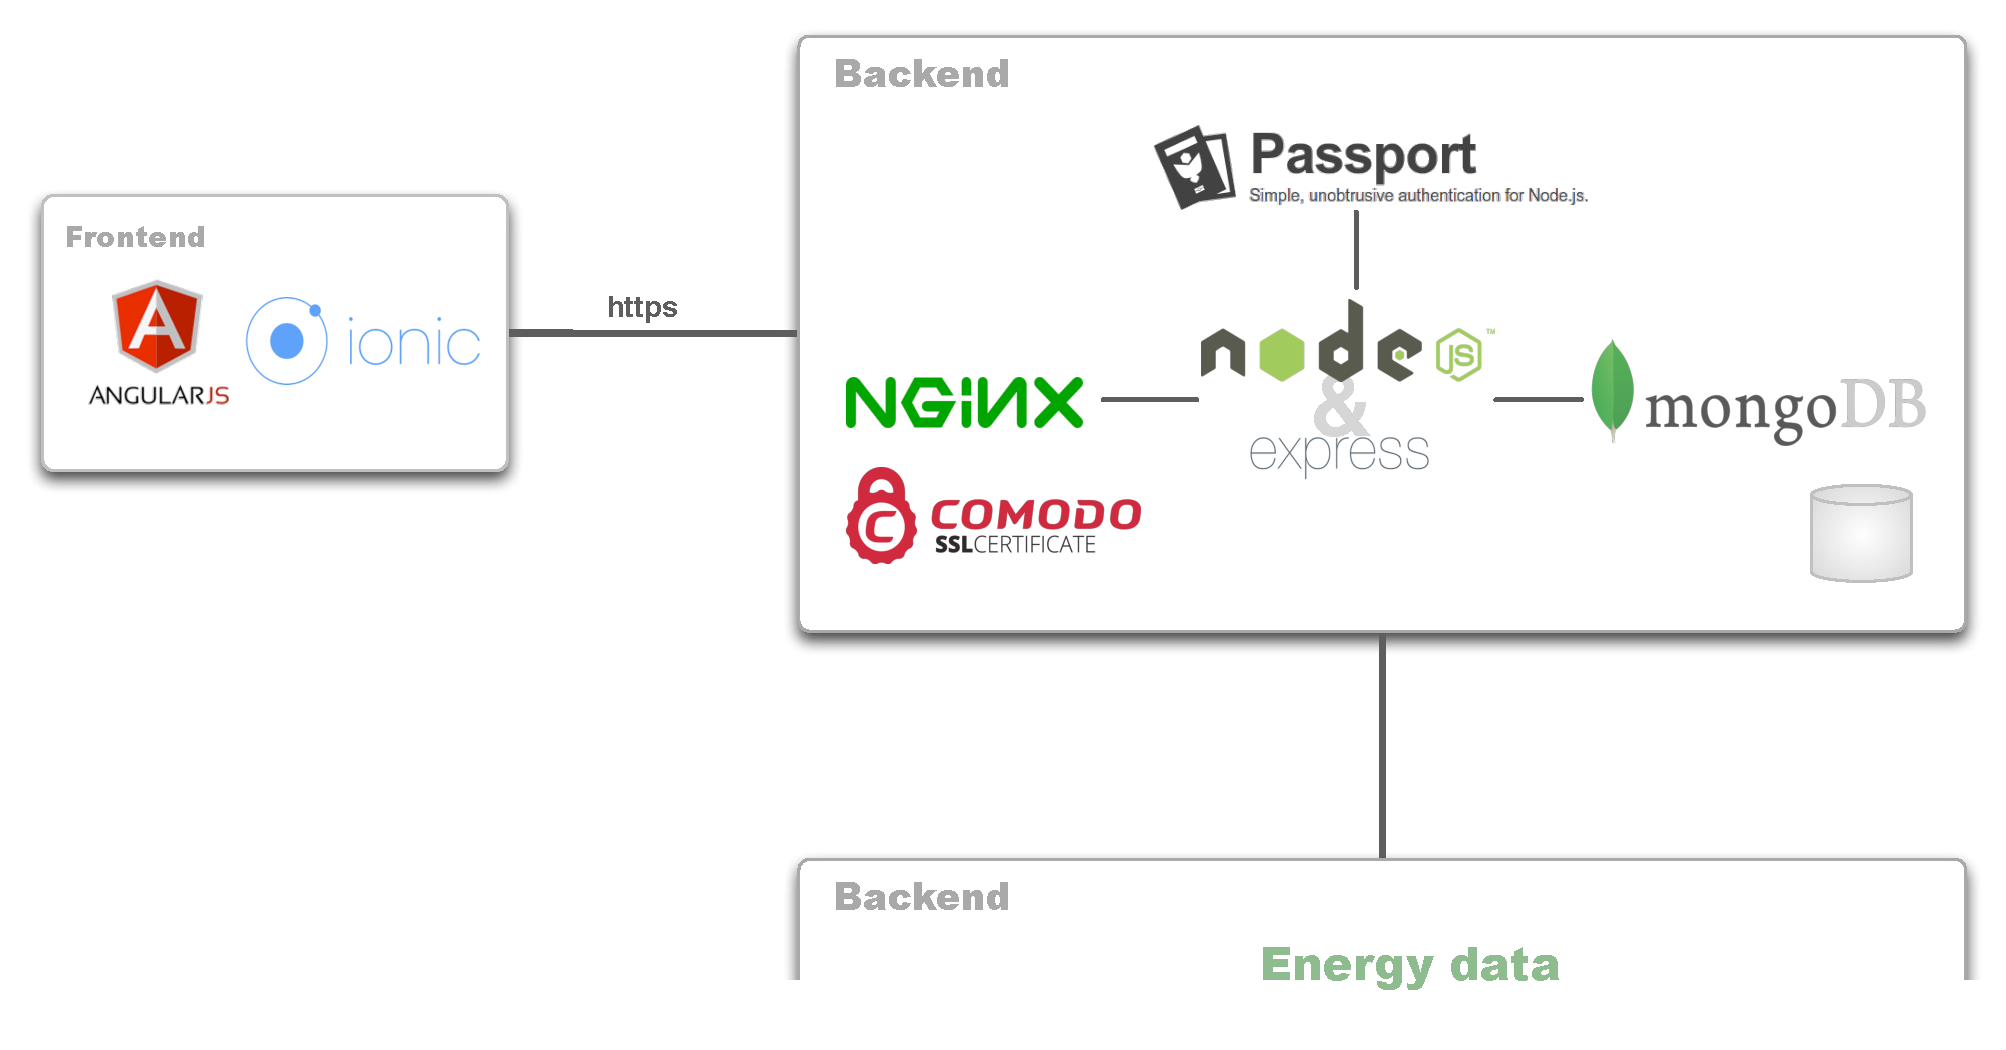
\includegraphics[width=0.9\linewidth]{img/architecture.pdf}
\caption{WP3 front-end and back-end overview (``Energy data'' is covered by WP4)}
\label{fig:ScreenShot2015-11-09at18}
\end{figure}

\subsection{CIVIS Front-end as a Hybrid Application} 

The CIVIS front-end (YouPower) is developed as a hybrid (cross-platform) mobile application using \textit{Ionic}\footnote{\url{http://ionicframework.com/}}, an HTML5 front-end development framework built with SASS\footnote{\url{http://sass-lang.com/}} and optimized for AngularJS\footnote{\url{https://angularjs.org/}} (a.k.a Angular). 
% 
The Ionic framework comes with native-styled mobile UI elements and layouts, and handles the look and feel and the UI interactions the app needs in order to be compelling\footnote{\url{http://ionicframework.com/docs/guide/}}. 

Angular as a JS framework provides directives (extensions of HTML attributes) and two-way data binding (binds input or output data of the view to a model) that simplify the app development with Model-View-Controller (MVC) architecture. 
In two-way data binding, the value of a data model is passed on from the view (or loaded from the back-end) to the controller at run-time, and the function in the controller returns the result (of the value manipulation) to the view. 
% 
Other noteworthy JS and Angular libraries (i.e. besides Ionic) we use for the front-end development are as follows:

\begin{itemize}

\item Highcharts\footnote{\url{http://www.highcharts.com/}}, a charting library in JS. It provides an easy way to add interactive charts to the application. 

\item Highcharts-ng\footnote{\url{https://github.com/pablojim/highcharts-ng}}, a simple Angular directive for Highcharts. 

\item Angular-translate\footnote{\url{https://angular-translate.github.io/}}, an Angular module for internationalization and localization of the application. (YouPower is currently available in English, Swedish and Italian.)

\item Angular-resource\footnote{\url{https://docs.angularjs.org/api/ngResource}}, an Angular module for interacting with RESTful server-side data sources. 

\item Underscore.js\footnote{\url{http://underscorejs.org/}}, a JS library that provides over 100 utility functions. 

\item Bootstrap-sass\footnote{\url{https://github.com/twbs/bootstrap-sass}}, a Sass-powered version of Bootstrap 3. 

\item Moment.js\footnote{\url{http://momentjs.com/}}, a JS library to parse, validate, manipulate and display dates. 

\item Ion-datetime-picker\footnote{\url{https://www.npmjs.com/package/ionic-datetime-picker}}, a date and time picker for the ionic framework. 

\end{itemize}


\subsection{CIVIS Back-end as a JS Runtime Environment}

The YouPower back-end is developed using the \textit{Node.js}\footnote{\url{https://nodejs.org/}} platform, a well-known JS based open source runtime environment for server-side applications. 
The platform is easily extensible and has a repository of libraries that support fast web development. 
% 
TU Delft prepared a virtual machine for CIVIS to host the WP3 back-end\footnote{\url{http://civis.tbm.tudelft.nl}}
using \textit{Nginx}\footnote{\url{https://nginx.org/en/}}, an http and reservse proxy server. 
% 
A \textit{Comodo}\footnote{\url{https://ssl.comodo.com/}} SSL certificate is installed on the server to provide secure communication (i.e. https). 

% 
The WP3 back-end interacts with the WP4 back-end, from which the former fetches relevant energy data that is particularly relevant for visualization of energy consumption/production and energy consumption signal. The availability of such data through the WP4 platform represents therefore a pre-condition for the ability of the app to correctly visualize such information.

\textit{MongoDB}\footnote{\url{https://mongodb.org/}} is used as the back-end database. It is document-oriented, and has flexible data schema and expressive query language. 
A list of the data models at the back-end can be found at {\footnotesize\url{https://github.com/CIVIS-project/YouPower/tree/master/backend/models}}. 
Figure~\ref{fig:datamodel} shows the data model schema.
%
\begin{figure}
\centering
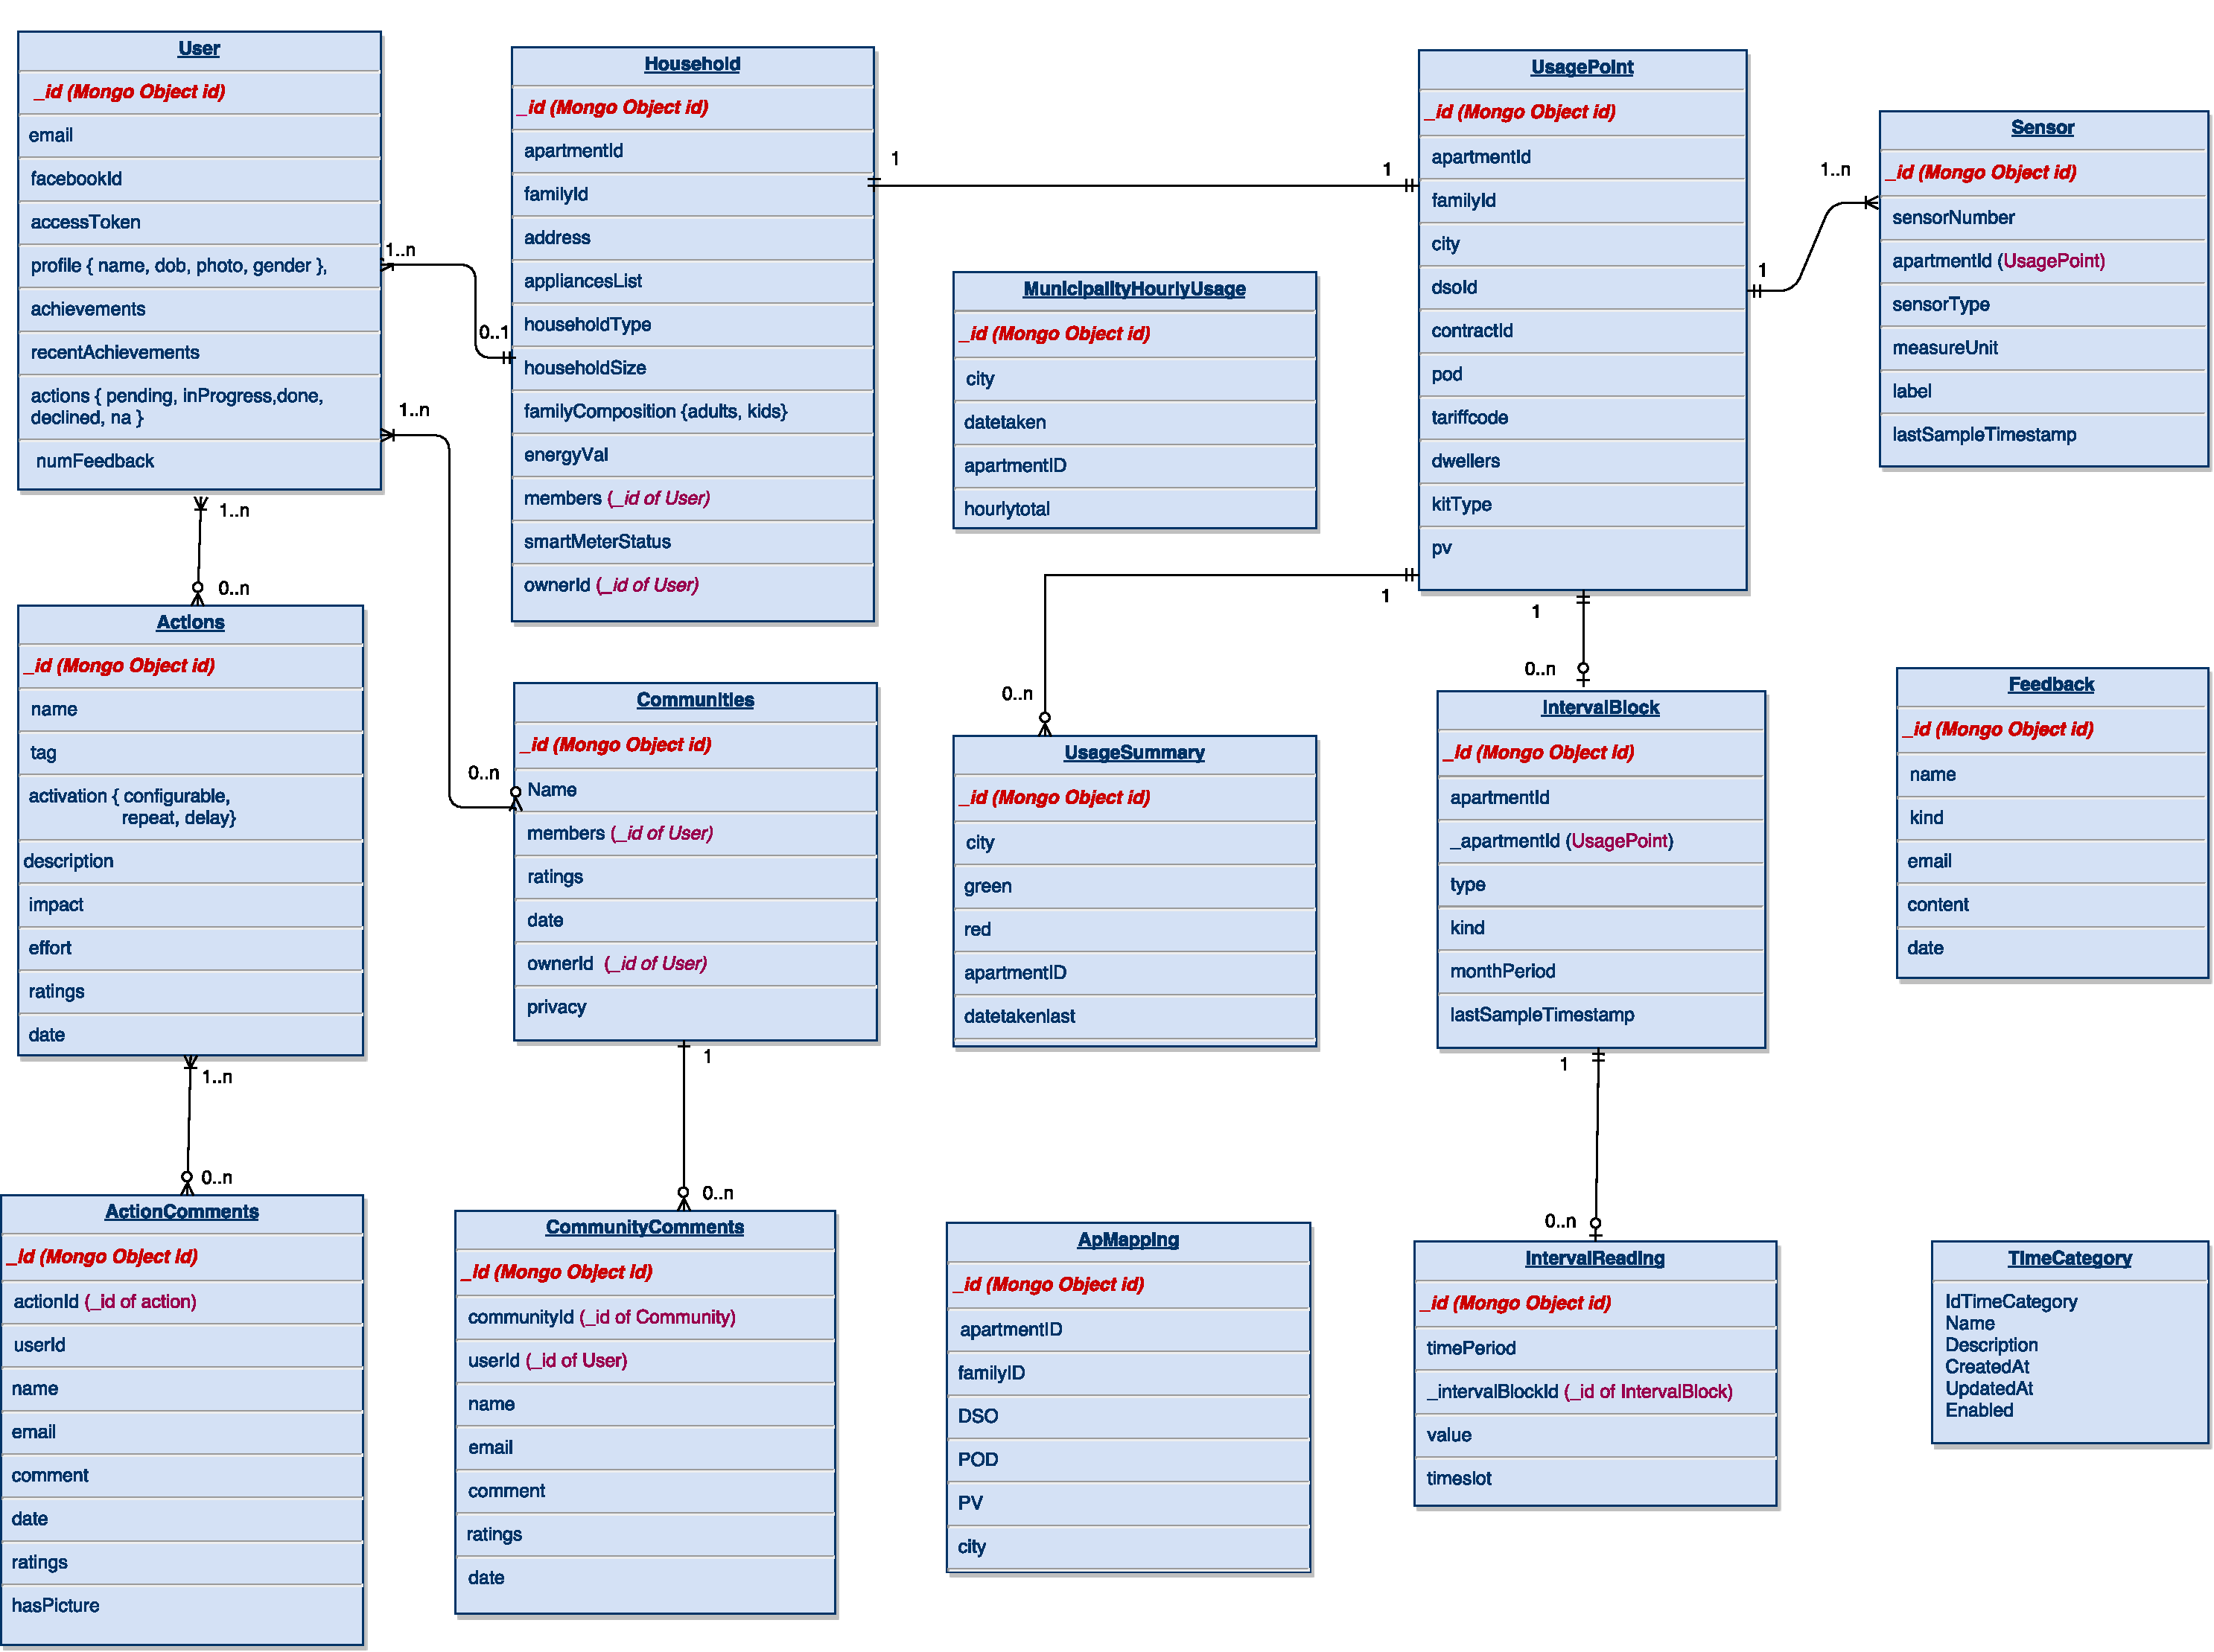
\includegraphics[height=.92\linewidth,angle=90]{img/7sdatamodel}
\caption{YouPower back-end data model schema}
\label{fig:datamodel}
\end{figure} 
% 

The noteworthy Node.js libraries used for the WP3 back-end development are as follows:

\begin{itemize}

\item Async.js\footnote{\url{https://github.com/caolan/async}}, which makes managing and combining asynchronous tasks easier. 

\item Express.js\footnote{\url{http://expressjs.com/}}, a Node.js application server framework we use as a basis for the REST API. 

\item Mocha\footnote{\url{https://mochajs.org/}}, a JavaScript unit test framework. 

\item Mongoose\footnote{\url{http://mongoosejs.com/}}, a MongoDB driver for Node.js. It provides a schema-based solution to model data. 

\item Passport.js\footnote{\url{http://passportjs.org/}}, for handling authentication of REST API requests for Node.js, both local (username password) and Facebook. 

\item Underscore.js\footnote{\url{http://underscorejs.org/}}, a JS library that provides over 100 utility functions. 
%\item Ionic Push\footnote{\url{https://apps.ionic.io/landing/push}}, for sending dynamic push notifications. 

\item Nodemailer\footnote{\url{https://nodemailer.com/}}, sending emails with Node.js.

\item Email-templates\footnote{\url{https://www.npmjs.com/package/email-templates}}, a Node.js module for rendering beautiful emails.

\item Fb\footnote{\url{https://www.npmjs.com/package/fb}}, a Node.js library for Facebook.

\item Moment.js\footnote{\url{http://momentjs.com/}}, a JS library to parse, validate, manipulate and display dates. 

\item APIDOC script\footnote{\url{http://apidocjs.com/}}, for inline documentation for the REST API. 
\item node-xml2js\footnote{\url{https://github.com/Leonidas-from-XIV/node-xml2js}}, Simple XML to JavaScript object converter. 
\item dateformat\footnote{\url{https://www.npmjs.com/package/dateformat}}, for formatting dates to custom formats. 
\item HTTPS\footnote{\url{https://nodejs.org/api/https.html}}, A nodeJs module used to make service calls over TLS/SSL. 
\item querystring\footnote{\url{https://www.npmjs.com/package/querystring}}, for deserializing querystring to an object. 
\item fs\footnote{\url{https://www.npmjs.com/package/querystring}}, for manipulating file in NodeJS. 
\end{itemize}

The YouPower back-end REST API documentation can be found at {\footnotesize\url{http://civis.tbm.tudelft.nl/apidoc/}}. 
% 

\subsection{Resources}


\section{User Registration Process}

In general, a user can sign up for a YouPower account at the application's welcome page\footnote{\url{https://app.civisproject.eu/frontend.html}}. In this case, the user can use the Action Suggestion part of the application. For the Housing Cooperative part or the Energy Awareness part of the application, more specific user (and energy) information is needed by the application. There are tailored solutions for the Swedish and the Italian test sites respectively which are presented in the following two subsections. 

\subsection{Swedish Test Site}

For the Swedish test site users, the registration process is as follows. 

\begin{enumerate}
\item A user receives a flyer with a URL that is housing-cooperative-specific, i.e. the housing cooperative which the user belongs to. 

The URL location is managed by KTH (i.e. it is a local Swedish URL) in the format of  \texttt{\small http://civis.proj.kth.se/}\textit{\{unique-link-of-a-housing-coopertive\}}. 

\item Through the URL, a user can reach a YouPower (Swedish user) sign up page that in addition to the inquiry of standard user information also asks for a unique identifier which allows to identify the user's household (and hence the associated energy data) with the user's permission. 

This is similar to but different from the Italian process where Italian test site users get their ApartmentID and HouseholdID beforehand. The Swedish process uses a unique ID of a user's electricity bill to identify different households. (Each user of a household still can register a separate user account at YouPower.) At the Swedish sign up page, there are also descriptions explaining how users can look up their IDs (which might be different for different housing cooperatives). 

\item The Swedish sign up page then asks for the user's household information, e.g. ...??? . 

\item After the registration, the page suggests the user to invite other household members via email.

\item At the end of the process, the user is directed to the housing cooperative view of the YouPower application. 

\end{enumerate}

\subsection{Italian Test Site}
New Trentino users should follow a 2 step process to use the full feature of YouPower.\\
\begin{enumerate}
\item A user will signup from YouPower \href{https://app.civisproject.eu/frontend.html#/welcome/}{home page} by filling up basic information(similar to swedish users). 
Users will then automatically be logged into YouPower after successful registration.
\item In order to access functionalities of the app which are discussed in Section  ~\ref{sec:energydata}, italian users should provide a valid \emph{ContractID} and \emph{Testbed Id}. Contract Id's will then be matched to ApartmentID of the household to access energy data from the backend while the testbed location will be used to fetch community related information like TOU signals in the municipality and  total consumption of the test site. At this step, the \emph{Energy Data} tab of YouPower will be activated for Trentino users.
\end{enumerate}
\section{Summary of WP3 Tasks Contribution}

\subsection{T3.1 Community Management}

Task 3.1 works in close cooperation with WP5 to explore community management. This is reflected in the diverse CIVIS platform functionalities in supporting housing cooperative activities in the Swedish test site (see Sec. \ref{sec:brf}) and the two local Consortia in the Italian test site respectively (see Sec. \ref{sec:energydata}). Those functionalities are designed and tailored to the local context as follows:   

\begin{itemize}
\item 
\end{itemize}

\subsection{T3.2 Energy Consumer Profiling}

This task was carried out between the last quarter of 2014 and the first quarter of 2015.
The goal was to provide a method to process individual electricity consumption
data in order to define a set of features that can characterize the behavioral patterns of each
consumer, and a way to group similar consumers together. The process devised can be summarized
as follows:

\begin{enumerate} 
\item Energy data is provided in XML format in the green button standard.

\item Energy data is stored into a MongoDB database.

\item The data is cleaned. In particular, missing data are detected and, where possible, interpolated. Outliers are detected and substituted with interpolated data. A report with all the modifications performed on
data is produced. 

\item Features are extracted from each individual energy consumption dataset. Examples of such
features are: average daily consumption, average hourly consumption, peak consumption, peak hour
consumption, total daily consumption. Each electric energy consumption time series is mapped to a
tuple of such features and stored in a MongoDB database.

\item Features tuples are clustered into similar groups. A range of algorithms are provided. These
algorithms are available in the scientific computing package \textit{scikit-learn}\footnote{\url{http://scikit-learn.org}}. Examples of those algorithms are K-means,
hierarchical clustering, affinity propagation, spectral clustering, DB scan.

\item A set of metrics to evaluate the goodness of the achieved clustering is provided. These metrics are implemented by scikit-learn. Examples of those are 
DBI (Davies-Bouldin Index),
CDI  (Cluster Dispersion Indicator),
MDI (Modified Dunn Index),
MSE (Mean Squared Error).
\end{enumerate}

The software is written in Python and it is available at the GitHub repository\footnote{\url{https://github.com/CIVIS-project/Consumer_profiling}}.

Note: after discussing with the CIVIS partners, we agreed that given the test site context of CIVIS, the consumption profiling part was not a most promising path towards load-shifting. Hence, although significant work has been done in this direction, we did not integrate this contribution to the YouPower application. (Nonetheless this contribution can still be useful for others.)
Instead, we devoted extra time and effort for the design and development of an energy production forecasting
system, Sec.~\ref{sec:energydata}, which can have a strong impact to help users achieve the load-shifting goals.

\subsection{T3.3 Interface with System Level}

The task 3.3 of CIVIS WP3 took care of exploring the different models for interconnecting the system level developed in WP4, the Energy ICT Platform, with the user level subsystem developed in WP3.

This work, performed between T02 and T08 of CIVIS project, was strictly in connection with the one performed in D4.3, where the interconnection of the two subsystems has been implemented and has been documented in D4.1, where the different models of interconnection have been described.

Sec. 8.3 of CIVIS D4.1 contains the descriptions of three different models that could be used in order to implement the connection between User Level and System Level:

\begin{itemize}
\item Solution 1: single connection and native HiReply MS SQL DB (Sec. 8.3.1 of D4.1);
\item Solution 2: single connection and use of a remote DB (Sec. 8.3.2 of D4.1);
\item Solution 3: double connection and use of a remote DB (Sec. 8.3.3 of D4.1).
\end{itemize}

Sec. 8.3 of D4.1 also describes the different features, in terms of scalability, that the three solutions can provide. For the deployment of CIVIS ICT Platform we adopted Solution 1, because it was suitable for achieving all the fixed goals in the provided project time frame and that is represented in Figure 1.

\subsection{T3.4 Energy Service Context}

This section highlights the lessons learned of business models for emerging social energy initiatives.
In its final deliverable (D6.3) work package 6 concludes with four main types of business models that can be applied to the CIVIS maturity scheme (depicting the development from emerging and promising to established energy initiative). 

\begin{itemize}
\item Efficiency Effects: becoming better at what you're doing - activities that enhance brand awareness and increase customer engagement.
\item Diversification: introducing products and services that are different that the initial domain of the organisation -- for (indirect) social as well as (longer term) financial benefits. 
\item Service Provisioning: facilitating others with available expertise -- providing available services at marginal costs to others.
\item Incubation: enabling innovation outside the organisation -- high(er) risk investment in the hope to achieve a financial or technical return on investment. 
\end{itemize}

Regardless of the specific maturity stage an organisation stage has achieved, of these four business model types, trying to achieve efficiency effects is one that is most applicable to any maturity stage. 

To that effect, the mobile energy app and the community platform that have been developed as part of this work package can be placed in this category. Both of these tools are prime examples of activities that enhance brand awareness and increase customer engagement in order to either make the members of the cooperatives more energy aware (and efficient) or that it convinces more inhabitants to join the cooperative.

As such these developments are (when introduced in the right way) powerful tools that can strengthen a chosen business model enormously. In work package 6 much attention has given to a step-by-step approach for (emerging) energy initiatives and particularly the use of tooling such as the business model canvas (bmc). The developed tools in work package three provides a solution for cooperatives to properly address their (mobile and online) members -- in other words, describing the ``channel'' element of the bmc.

Examples of this have become apparent in surveys with the board members of the testsites in Sweden and Italy. What CIVIS learned is that there is a distinct advantage in having a (ICT) collaboration or (ICT) information solution available to the cooperative members. While it does not come as a surprise that providing members with information on energy generation, consumption and saving does increases awareness -- it is the extent of the impact on awareness that interests us.

While initial uptake of the CIVIS apps has been slow, once people started to use it the awareness of what is happening within the cooperative as a whole is certainly increasing. Though not statistical relevant, several board members have remarked increased feedback from members since making the mobile apps available. For leadership, this kind of feedback and interaction is particularly helpful terms of gauging if certain initiatives have a positive effect within the cooperation. In a sense this contributes more to their understanding than just looking at the amount of website ``hits'' that are available through the IT responsible department or person. It is a combination of context and hard numbers that makes the learning process possible in the first place. 

\section{Conclusion}

The main activities of WP3 in the 3rd year of the CIVIS project were carried out to continue and complete the design and development of the CIVIS platform, called YouPower, to meet the project goal and to suit the context and objective of the test sites' use cases. 
We continued the adaptive agile development process, and expanded upon the results from the 2nd year of the CIVIS project. The design of YouPower is composed of a set of features that can be divided into three interrelated parts: 
\begin{enumerate}
\item Action suggestions, where users are provided with suggestions of  actions that are implementable in everyday household practices. Users are presented with motivators for behavior change (and its process), and means for self-monitoring, self-reflection and social sharing of the pro-environmental behavior change process at individual, household and community levels.

\item Housing cooperatives, where energy management and cooperative energy reduction actions are linked to each cooperative's energy performance (and building level energy information). YouPower allows comparison between housing cooperatives based on the energy performance and actions, and supports knowledge exchange and social sharing and learning among cooperatives in energy reduction actions.

\item Energy awareness, where users are presented with real time and historical energy consumption and production information at individual and comparative (community) level, and are provided with time-of-use signals based on real time and forecasted information about local production from renewable sources and the corresponding energy demand in order to enable load-shifting actions in everyday practice. 

\end{enumerate}

Along the design of those features, we developed ten design guidelines that address a number of design issues emerged from the CIVIS YouPower project. These guidelines are based on literature about pro-environmental intervention and social and environmental psychology combined with our design experience, and can be useful for the design of other energy community and applications for pro-environmental interventions. 

The CIVIS YouPower platform is deployed at the Stockholm (Sweden) and Trento (Italy) test sites:  the first deployment at the Stockholm test site was in Nov 2015 and Trento test site in Mar 2016 correspondingly, and since then the production server had been updated once there were new parts ready for deployment. WP3 uses two ways to monitor YouPower user activities: (1) the API calls to the WP3 CIVIS server are logged into WP3 YouPower database; (2) the important user actions (i.e., user clicks) in the YouPower app are logged  through \textit{MixPanel}\footnote{\url{https://mixpanel.com/}}.
As agreed during the 2nd year's CIVIS review meeting in Brussels, the CIVIS project team will continue the YouPower data collection (keep the servers running) for 6 months after the end of the project. 

In principle, any interested users (also those outside of the test sites) can sign up the YouPower application. The Action Suggestion part of the application is ready to be used as-is. The Housing Cooperative part is applicable to energy management works of housing cooperatives/associations that exist in a number of EU and non EU countries. The cooperative energy performance feature requires energy consumption data at cooperative level. The Energy Awareness part of the application requires access to users household energy consumption and production (if applicable) data. At the CIVIS test sites, the required energy data at cooperative, household and individual appliance levels are collected by smart meters and smart plugs/sensors. The details about energy data accessibility often differ from case to case, hence requires some adaptation. 

As stated in an earlier deliverable, designing well is not easy \citep{Norman2002}: if a product is truly new, it is unlikely that anyone will know how to design it right at the first time.  
The design and development of YouPower together with user studies at the Swedish and Italian test sites by the CIVIS project formed a good basis for and provided valuable insights into the social dimension of the energy network to achieve sustainable energy goals. This is a first step towards long-term sustainable socio-technical development.  
CIVIS partners are looking for opportunities, i.e. new research projects, to bring the result of this project into further steps. The CIVIS project has its results and the source of the YouPower application open to the public, which may bring future endeavors of interested communities to explore and expand upon the current effort towards promoting sustainable social energy actions. 







\section*{References}
\addcontentsline{toc}{section}{References}
\bibliographystyle{chicagoa}

\begingroup
\renewcommand{\section}[2]{}
\setlength{\bibsep}{0pt}
    \linespread{1}\selectfont
\bibliography{bib,sanja}
\endgroup

\end{document}
